% IWAI 2026 submission: Springer LNCS format, max 12 pages (incl. figures,
% excl. references) + appendix of up to 12 pages, double-blind.
\documentclass[runningheads]{llncs}

% ---------- encoding & fonts ----------
\usepackage[T1]{fontenc}
\usepackage[utf8]{inputenc}
\usepackage[expansion=false]{microtype}

% ---------- math ----------
\usepackage{amsmath}
\usepackage{amssymb}
\usepackage{mathtools}

% ---------- figures ----------
\usepackage{graphicx}
\graphicspath{{figures/}}
\usepackage{tikz}
\usetikzlibrary{calc,positioning,arrows.meta}
\usepackage{subcaption}
\usepackage{xcolor}

% ---------- layout ----------
% (LNCS fixes the text block; geometry must not be loaded)
\usepackage[numbers,sort&compress]{natbib}
\usepackage{hyperref}
\hypersetup{hidelinks}

% ---------- shorthands ----------
\newcommand{\KL}[2]{D_{\mathrm{KL}}\!\left[#1\,\middle\|\,#2\right]}
\newcommand{\E}[1]{\mathbb{E}\!\left[#1\right]}
\newcommand{\Eq}[2]{\mathbb{E}_{#1}\!\left[#2\right]}
\newcommand{\Var}[2]{\mathrm{Var}_{#1}\!\left[#2\right]}
\newcommand{\desc}{\mathrm{desc}}
\newcommand{\rw}{\rightsquigarrow}
\newcommand{\Top}{\mathsf{T}}          % propagation operator
\newcommand{\bone}{\mathbf{1}}         % unit source vector

% ---------- palette ----------
\definecolor{costc}{RGB}{40,80,170}
\definecolor{newc}{RGB}{200,120,30}      % proposed / new node (amber)

% ---------- network figure macros ----------
\tikzset{
  bel/.style={circle,draw=black!70,line width=0.4pt,minimum size=7mm,inner sep=0pt,font=\small},
  obs/.style={rectangle,draw=black!45,fill=white,minimum size=2.6mm,inner sep=0pt},
  core/.style={line width=0.9pt,black!75},
  belt/.style={line width=0.5pt,black!55},
  sens/.style={dashed,line width=0.4pt,black!40},
  anno/.style={font=\scriptsize\itshape,text=black!75,align=center},
  annoarrow/.style={-{Stealth[length=1.4mm]},line width=0.3pt,black!55},
  % directed dependency edges; the *c variants shorten to clear 7mm nodes drawn at coordinates
  dcore/.style={-{Stealth[length=1.5mm]},line width=0.9pt,black!75},
  dbelt/.style={-{Stealth[length=1.3mm]},line width=0.5pt,black!55},
  dcorec/.style={dcore,shorten <=0.37cm,shorten >=0.37cm},
  dbeltc/.style={dbelt,shorten <=0.37cm,shorten >=0.37cm},
}
\newcommand{\Positions}{%
  \coordinate (A) at (0,1.1);   \coordinate (B) at (-1.1,0);
  \coordinate (C) at (1.1,0);   \coordinate (D) at (0,-1.1);
  \coordinate (b1) at (-1.45,1.95); \coordinate (b2) at (1.45,1.95);
  \coordinate (b3) at (-2.25,0);    \coordinate (b4) at (2.25,0);
  \coordinate (b5) at (-1.45,-1.95);\coordinate (b6) at (1.45,-1.95);
  \coordinate (o1) at (-1.95,2.6);  \coordinate (o2) at (1.95,2.6);
  \coordinate (o3) at (-3.1,0);     \coordinate (o4) at (3.1,0);
  \coordinate (o5) at (-1.95,-2.6); \coordinate (o6) at (1.95,-2.6);
}
\newcommand{\Edges}{%
  \draw[dcorec] (A)--(B); \draw[dcorec] (A)--(C); \draw[dcorec] (A)--(D);
  \draw[dcorec] (B)--(C); \draw[dcorec] (B)--(D); \draw[dcorec] (C)--(D);
  \draw[dbeltc] (A)--(b1); \draw[dbeltc] (A)--(b2);
  \draw[dbeltc] (B)--(b3); \draw[dbeltc] (C)--(b4);
  \draw[dbeltc] (D)--(b5); \draw[dbeltc] (D)--(b6);
  \draw[sens] (b1)--(o1); \draw[sens] (b2)--(o2); \draw[sens] (b3)--(o3);
  \draw[sens] (b4)--(o4); \draw[sens] (b5)--(o5); \draw[sens] (b6)--(o6);
  \node[obs] at (o1){}; \node[obs] at (o2){}; \node[obs] at (o3){};
  \node[obs] at (o4){}; \node[obs] at (o5){}; \node[obs] at (o6){};
}
% tiny 3-node paradigm DAG inside an agent circle at (#1,#2)
\newcommand{\miniNet}[2]{%
  \draw[black!70,line width=0.5pt,fill=white] (#1,#2) circle (0.46);
  \fill[costc!75] ($(#1,#2)+(0,0.22)$) circle (0.055);
  \fill[costc!75] ($(#1,#2)+(-0.22,-0.13)$) circle (0.055);
  \fill[costc!75] ($(#1,#2)+(0.22,-0.13)$) circle (0.055);
  \draw[costc!80,line width=0.4pt,-{Stealth[length=1mm]}] ($(#1,#2)+(0,0.22)$) -- ($(#1,#2)+(-0.22,-0.13)$);
  \draw[costc!80,line width=0.4pt,-{Stealth[length=1mm]}] ($(#1,#2)+(0,0.22)$) -- ($(#1,#2)+(0.22,-0.13)$);
  \draw[costc!80,line width=0.4pt,-{Stealth[length=1mm]}] ($(#1,#2)+(-0.22,-0.13)$) -- ($(#1,#2)+(0.22,-0.13)$);
}

% ======================================================================
\title{Paradigm Shifts: Motivated Inference on Webs of Belief}
\titlerunning{Motivated Inference on Webs of Belief}
% ----- ANONYMIZED for double-blind review. Restore for camera-ready: -----
% \author{Jonas Hallgren\inst{1} \and David Hyland\inst{2} \and Mahault Albarracin\inst{3}}
% \authorrunning{J. Hallgren et al.}
% \institute{Affiliation 1 \email{...} \and Affiliation 2 \and Affiliation 3}
\author{Anonymous Submission}
\authorrunning{Anonymous Submission}
\institute{Anonymous Institution(s)}
% ======================================================================

\begin{document}
\maketitle

\begin{abstract}
Paradigm shifts are a significant driver of belief revision in scientific communities.
Peripheral commitments drift gradually under accumulating evidence, while central commitments
resist revision even when evidence is against the theory---and when they do change, they
change quickly. We study this phenomenon within an active inference framework, building on
recent accounts that recast belief updating as motivated inference subject to a cost of
changing one's mind. Drawing on Lakatos and Kuhn, we represent an agent's theoretical
commitments as a directed network of interdependent beliefs, in which the cost of revising a
commitment depends both on standing affective commitments and on how much surrounding
inference must re-equilibrate when it moves---so the hard core and protective belt fall out
of the precision geometry rather than being decreed. Agents exchange beliefs, and pieces of
structure, over a communication network. Characterising the resulting dynamics analytically
and through simulation, we find that the field's default aggregation step---precision-weighted
averaging---cannot reproduce the signature of paradigm change: it contracts the community onto
a compromise network no member holds, whatever the parameters. We then construct the
representational capacity the default lacks---a posterior over rival structures within each
agent---and show that it recovers the Kuhn cycle, with crisis as a measurable state of the
belief: normal science, crisis, revolution, new normal. We close by discussing implications
for engineered communities of reasoning agents, whose aggregation protocols decide the same
question by design.

\keywords{Active inference \and Structure learning \and Belief sharing \and Paradigm change \and Social epistemology}
\end{abstract}

% ======================================================================
\section{Introduction: changing a frame, not a credence}
\label{sec:background}
% ======================================================================

If we want science to keep going well, we need to know how it \emph{works}: what kind of agent
can do science at all, how a community comes to represent a new dimension of the
world, and how it loses information it once held. The question has a second audience, because
communities of reasoning agents are now \emph{built} as well as studied, and every such
community commits, in its aggregation step, to an answer it rarely examines: what happens to
the member who disagrees. Machine learning names the property at stake \emph{open-endedness}
\citep{stanley2017oe,hughes2024}; social epistemology catalogues its failure modes
\citep{nguyen2018,zollman2010}. What neither supplies is a foundation: a model of a
\emph{community} of structure-learning agents explicit enough that one can prove which
aggregation dynamics preserve open-endedness and which foreclose it. This paper tries to be a
step towards that foundation. We show that the most natural baseline---Gaussian beliefs under
precision-weighted pooling---provably lacks the capacity, and we construct a way for it to
have that capacity. The problem, throughout, is averaging: taking the mean refines the frame
everyone shares, and can never grow a new one.

To change one's mind about a fact is to update a belief; to change a paradigm is to change the
\emph{frame} in which beliefs are posed---not a credence but a \emph{structure}, a network of
conditional dependencies through which information propagates. This is the phenomenon Kuhn
named but could not formalise \citep{kuhn1962}: nothing in \emph{The Structure of Scientific
Revolutions} says, mechanistically, why a community holds a structure of commitments past the
first disconfirming evidence, nor what finally makes the holding give way. Take an example:
when the chemical community of the late eighteenth century gave up phlogiston, it did not
revise a single credence: it rewrote a network in which combustion, calcination, respiration,
and the theory of acids were all load-bearing on a hub that had to go
\citep{blumenthal2017,holmes2000,boantza2011}. Phlogiston was load-bearing for too much.

We can model such communities with network epistemology, the dominant formalism for them---but
in its naive form, a scalar credence in a fixed proposition updated on a trust graph
\citep{zollman2010,oconnor2019,zollman2013,jonard2025,michelini2023}, it cannot represent
structure learning. The phlogiston puzzle
is not a failure to converge on a number---the commitments were \emph{entangled}, and the
dispute was over which entanglements to keep. Thagard's ECHO \citep{thagard1989,thagard1990}
captures the structural intuition as undirected coherence but lacks the directed dependencies
and the carry-over cost of mind-change derived below; active-inference accounts supply precision-based
lock-in \citep{albarracin2022}, warnings that naive aggregation degrades collective precision
\citep{friston2023federated,waade2025}, and a single-agent variational cost of mind-change
\citep{hyland2025}. What none of these does is make \emph{belief structure itself} the object
of inference: a scalar credence can never say how revising one commitment forces a re-reading
of the rest---agents can herd on a number or split over it, but they cannot come to hold
different \emph{kinds} of world.

This paper lets a piece of \emph{structure} travel, so that one agent can come to represent a
commitment its peers do not. Its agents carry a directed network of commitments and learn that
network by Bayesian model \emph{reduction}---and by reduction only: expansion is deferred by
scope (\S\ref{sec:structurelearning}), but when agents are \emph{given} new structures, they
can incorporate them into their own system. They are \emph{bounded}, sampling a complex
world through narrow channels, valuing some conclusions over others, and judging what they
receive against their own model. Section~\ref{sec:bmebmr} assembles this community from the
field's own default choices; Section~\ref{sec:results} shows what those defaults force---pooling is a
contraction, so a conflicting source is never rejected, only averaged in---and what undoes it:
agents that represent rival structures keep different readings of the same world apart, and
run the Kuhn cycle with crisis as a state of the belief. The discussion
draws the map: what filling the representational slot bought, and what
remains.

% ======================================================================
\section{Desiderata for a structural model of science}
\label{sec:hidden}
% ======================================================================

A structural model of science needs at least three ingredients. First, \emph{structure as the
object of inference}: a scientist confronting a
new domain is not given the right variables, let alone the dependencies among them; frames
differ in kind, not in degree, so credences over a fixed menu cannot carry them
\citep{ullman2020,kemp2008form,ullman2012}. Active inference can model this: \emph{when}
structure is the object of inference, exploration need not be added by hand, as the
$\epsilon$ of an $\epsilon$-greedy algorithm is
\citep{zollman2010,oconnor2019}; it can be cast as the epistemic value of \emph{expanding} the
model to entertain a commitment not yet in it \citep{friston2015,friston2017curiosity}, with
Bayesian model reduction as its complement, pruning what the data abandon in closed form
\citep{friston2018bmr,neacsu2022}. To model structure learning, then, is to model how a Bayes
net learns to change \emph{itself} over time.

\emph{Value}, or motivated belief updating: the underlying values and biases a scientist
already has about what they care about. A result on which a career rests
is held more tightly than its evidence warrants \citep{kitcher1990,strevens2003}, and attitudes
demonstrably live on networks of exactly this kind \citep{dalege2016}. And \emph{communication},
because science is social: beliefs travel a trust graph and must somehow be combined when they
meet. Each requirement has a default formalization, so natural it is hardly ever examined.
Beliefs over a network become a precision-weighted Gaussian model; value becomes a utility that
tilts the prior \citep{hyland2025}; combination becomes precision-weighted averaging, the
information form of classical opinion pooling \citep{degroot1974,genest1986}.
Section~\ref{sec:bmebmr} builds the community out of exactly these defaults, on purpose. The
question the rest of the paper asks is whether such a community can ever do more than
\emph{refine}: whether agents built this way can grow a frame, and not merely polish the one
they hold.

% ======================================================================
\section{The model}
\label{sec:bmebmr}
% ======================================================================

We draw the system whole first---a population of agents on a trust graph---then build the single
agent up from first principles, and finish by stating the dynamics as an explicit per-round loop
(\S\ref{sec:model}).

\subsection{The population, and the paradigm network each agent carries}
\label{sec:carryover}

We turn to the third requirement, communication, first. A population of $N$ agents inhabits a
shared hidden world. Agents are
coupled on a trust graph: communities are blocks of a stochastic block model, with dense
intra-community edges and an inter-community coupling weight (\emph{inter}) that we sweep from
total isolation to dense contact. Each agent privately carries its own \emph{paradigm network}, a directed graph
$G=(V,E,\Pi)$: nodes carry theoretical commitments $x_v$, edges carry inferential dependencies,
and each edge bears a coupling precision $\pi_{uv}$ measuring how tightly $v$ is bound to $u$.
The network is just a generative model whose hidden states are the commitments themselves:
internal coherence is the precision-weighted graphical model
$p(x\mid G)\propto\prod_{(u\to v)\in E}\psi_{uv}(x_u,x_v)^{\pi_{uv}}$, from which the agent's
conservatism and conviction will be derived (Eqs.~\ref{eq:kappa}
and~\ref{eq:U} below). Figure~\ref{fig:population} draws the picture.

\begin{figure}[h!]
\centering
\resizebox{0.68\linewidth}{!}{%
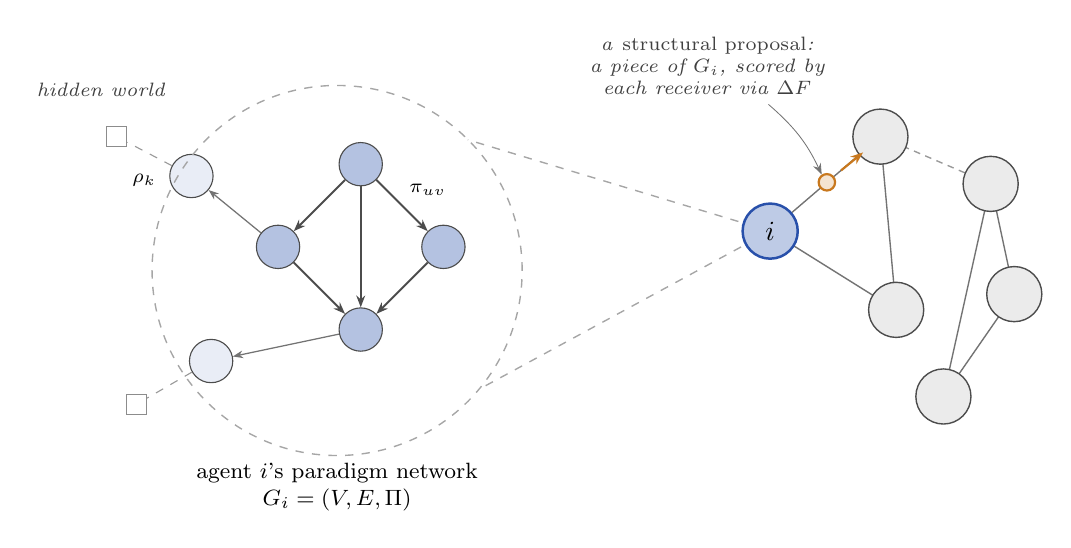
\begin{tikzpicture}[
  n/.style={circle,draw=black!70,line width=0.4pt,fill=costc!35,minimum size=5.5mm,inner sep=0pt},
  nb/.style={circle,draw=black!70,line width=0.4pt,fill=costc!10,minimum size=5.5mm,inner sep=0pt},
  ag/.style={circle,draw=black!70,line width=0.5pt,fill=black!8,minimum size=7mm,inner sep=0pt},
  dep/.style={-{Stealth[length=1.5mm]},line width=0.7pt,black!70},
  depb/.style={-{Stealth[length=1.3mm]},line width=0.45pt,black!55}]
  % ---- left: agent i's paradigm network, magnified ----
  \node[n] (A) at (0,1.05) {};
  \node[n] (B) at (-1.05,0) {};
  \node[n] (C) at (1.05,0) {};
  \node[n] (D) at (0,-1.05) {};
  \node[nb] (b1) at (-2.15,0.9) {};
  \node[nb] (b2) at (-1.9,-1.45) {};
  \draw[dep] (A)--(B); \draw[dep] (A)--(C); \draw[dep] (A)--(D);
  \draw[dep] (B)--(D); \draw[dep] (C)--(D);
  \draw[depb] (B)--(b1); \draw[depb] (D)--(b2);
  \node[obs] (o1) at (-3.1,1.4) {};
  \node[obs] (o2) at (-2.85,-2.0) {};
  \draw[sens] (b1)--(o1); \draw[sens] (b2)--(o2);
  \node[font=\scriptsize] at (0.85,0.72) {$\pi_{uv}$};
  \node[font=\scriptsize] at (-2.75,0.85) {$\rho_k$};
  \node[anno] at (-3.3,2.0) {hidden world};
  % the agent's boundary, pierced by its sensory channels
  \draw[black!35,dashed,line width=0.5pt] (-0.3,-0.3) circle (2.35);
  \node[font=\footnotesize,align=center] at (-0.3,-3.05)
    {agent $i$'s paradigm network\\$G_i=(V,E,\Pi)$};
  % ---- magnifier lines to one agent of the trust graph ----
  \draw[black!35,dashed,line width=0.5pt] (5.2,0.2) -- (1.36,1.36);
  \draw[black!35,dashed,line width=0.5pt] (5.2,0.2) -- (1.5,-1.81);
  % ---- right: the trust graph, two communities ----
  \draw[belt] (5.2,0.2)--(6.6,1.4); \draw[belt] (5.2,0.2)--(6.8,-0.8);
  \draw[belt] (6.6,1.4)--(6.8,-0.8);
  \draw[belt] (8.0,0.8)--(8.3,-0.6); \draw[belt] (8.3,-0.6)--(7.4,-1.9);
  \draw[belt] (8.0,0.8)--(7.4,-1.9);
  % the single weak channel between communities
  \draw[line width=0.5pt,black!40,dash pattern=on 2.4pt off 2pt] (6.6,1.4)--(8.0,0.8);
  \node[ag,fill=costc!30,draw=costc,line width=0.9pt] (ai) at (5.2,0.2) {$i$};
  \node[ag] (a2) at (6.6,1.4) {};
  \node[ag] (a3) at (8.0,0.8) {};
  \node[ag] (a4) at (6.8,-0.8) {};
  \node[ag] (a5) at (8.3,-0.6) {};
  \node[ag] (a6) at (7.4,-1.9) {};
  % ---- the object being passed: a structural proposal ----
  \node[circle,draw=newc,line width=0.8pt,fill=newc!20,inner sep=2.1pt] (prop) at (5.92,0.82) {};
  \draw[-{Stealth[length=1.6mm]},newc,line width=0.8pt] (6.1,0.97) -- (6.38,1.2);
  \node[anno] (anProp) at (4.4,2.3) {a \emph{structural proposal}:\\a piece of $G_i$, scored by\\each receiver via $\Delta F$};
  \draw[annoarrow] (anProp) to[bend left=12] (prop);
\end{tikzpicture}}
\caption{The population model. Right: a trust graph, fixed at the start (stochastic block
model)---dense channels within a community, one weak weight \emph{inter} between. Left,
magnified: each agent's private paradigm network $G_i=(V,E,\Pi)$, its belt reading the hidden
world through channels of precision $\rho_k$. Along trust channels travel fused posteriors and
\emph{structural proposals}: pieces of paradigm each receiver scores against its own net by
$\Delta F$ (Eq.~\ref{eq:bmr}).}
\label{fig:population}
\end{figure}

Two kinds of things propagate on this underlying network. Beliefs and accumulated precisions
are fused across trust edges in information form---an agent's own evidence and its neighbours'
weighted in proportion to trust, the information-form counterpart of trust-weighted averaging
in opinion dynamics \citep{degroot1974,acemoglu2011}. And---not standard---\emph{structure}
spreads the same way: a neighbour's newly awakened node arrives as a proposal, scored against
the receiver's own model (\S\ref{sec:structurelearning})---not only a number but a piece of
structure, evaluated against wiring the sender does not see.

To see what one of those private networks holds, let us take an example. The
phlogiston paradigm, at its smallest, is three commitments wired together:
combustion releases phlogiston; calcination is combustion, slowed; respiration is combustion,
tamed. Each commitment conditions the next, evidence for any one bears on all, and the question
``what if the calx \emph{gains} weight?'' has no local answer---it tugs the whole web. A
paradigm, in this paper, is that web made explicit.

Concretely, $p(x\mid G)$ is a linear-Gaussian structural equation model in the lineage of
Wright's path analysis \citep{wright1934}, edges as path coefficients and precisions as their
weights; we work throughout in that regime, which puts every quantity below in closed form
(Appendix~\ref{app:operator}). Two stipulations: agents are \emph{honest}---no one misreports,
so lock-in is never a dishonesty artifact---and \emph{bounded}, minimizing variational free
energy step by step \citep{dacosta2020}---that is, they do not plan over longer horizons; they
are myopic.

What we model is that revising a commitment is not a local act: changing $x_v$ forces
everything downstream of it to re-equilibrate, along every chain of dependence. If $A$ is the
matrix of edge precisions, summing chains of every length gives $\sum_k A^k=(I-A)^{-1}$, a
finite sum on a DAG (an object path analysis and network science already own
\citep{wright1934,bollen1987,katz1953,bonacich1987,malioutov2006}). We adopt it as the
\emph{propagation operator}
$\Top=(I-A)^{-1}$: the entry $\Top_{iw}=\pi_{i\rw w}$ is the total precision-weighted coupling
propagated from $i$ to $w$ along all directed paths (Appendix~\ref{app:operator}).

Conservatism is then recognized rather than posited. Place a unit of weight on every node and ask,
for each commitment $i$, how much total weight a revision of $i$ would disturb. That is the operator
applied to the unit source,
\begin{equation}
\kappa \;=\; \Top\,\bone,
\qquad
\kappa_i \;=\;1+\!\!\sum_{w\in\desc(i)}\!\!\pi_{i\rw w},
\label{eq:kappa}
\end{equation}
the precision-weighted mass of a node's descendants. In network-science terms this is a
centrality (the broadcast Katz index), usually read as influence or status; we read the same
number as \emph{revision cost}---a commitment is exactly as expensive to revise as the mass that
must re-equilibrate when it moves. Conservatism is a centrality the graph already determines,
not a disposition assigned by hand; one can read $\kappa_i$ almost as a momentum or inertia
term: the older and more central a commitment, the more mass moves with it.

What we add to this inherited machine comes in two layers. The first is contact with the world. The
dense, high-precision interior of the network is the \emph{core}; the sparse periphery in contact
with observation is the \emph{belt}, each belt node reading the world through a sensory channel of
precision $\rho_k$---Lakatos's hard core and protective belt \citep{lakatos1970}, here
determined by the precision geometry rather than decreed. The central nodes are coupled to
many more nodes; in our model, these are the \emph{axioms} of the scientific system. The core
carries no direct sensory
channel: an interior commitment is revised only by error propagated inward from the belt,
through the same operator---costly by Eq.~\eqref{eq:kappa} and insulated by position, which is
what makes it slow.

The second layer is value, and the operator is run twice. This is the second desideratum of
\S\ref{sec:hidden}---motivated belief updating: scientists hold values and biases about what
they care about, and a model of science has to represent them. We attach to each node an
intrinsic utility $u_i$ and let it propagate
through the \emph{same} operator: a commitment one wants true lends value to its dependents, so the
conviction field is
\begin{equation}
U \;=\; \Top\,u,
\qquad
U_i \;=\; u_i+\!\!\sum_{w\in\desc(i)}\!\!\pi_{i\rw w}\,u_w .
\label{eq:U}
\end{equation}
In the operator's path-analytic reading, $U$ is the total effect of wanting things true. Where the
inherited models propagate a single source, a paradigm carries two: $\Top\bone$ and $\Top u$ are
linearly independent unless $u\propto\bone$, so the two fields need not align---a commitment can
be central yet value-neutral, cheap yet strongly held (Fig.~\ref{fig:twofields},
Appendix~\ref{app:operator}).

\subsection{Motivated revision, structure learning, and forgetting}
\label{sec:revision}

The bounded agent revises its belief $q(x)$ over the whole network by a motivated trade
\citep{hyland2025}: the variational cost of changing its mind---divergence from the prior its own
Bayes net encodes---against accuracy to the evidence and the value of where the commitments land,
\begin{equation}
\begin{aligned}
\mathcal{F}[q]\;&=\;
\underbrace{\KL{q(x)}{p(x\mid G)}}_{\text{mind-change cost}}
\;-\;\underbrace{\Eq{q}{\log p(o\mid x,G)}}_{\text{accuracy}}
\;-\;\lambda\,\underbrace{\Eq{q}{U^{\!\top}\!x}}_{\text{value}}\\[2pt]
&\Longrightarrow\qquad
q_\lambda(x)\;\propto\;p(x\mid o,G)\,e^{\lambda\,U^{\!\top}\!x},
\end{aligned}
\label{eq:tilted}
\end{equation}
with $\lambda$ a single temperature governing how far value may bend the evidence. The KL is
anchored to the \emph{network prior}: mind-change is priced from where the mind currently
stands, in the metric of the paradigm's own precision (Appendix~\ref{app:operator},
Eq.~\ref{eq:mindcost}), and the minimizer is classical---the exponential tilt KL-regularized
utility maximization always yields \citep{todorov2009,ortega2013}. What is ours is the source
of the tilt, a conviction field propagated through the paradigm's own operator. In the
linear-Gaussian regime the tilt is a pure mean shift: value displaces where the commitments
come to rest (by $\lambda\Sigma U$) and leaves the uncertainty untouched. What opposes the
displacement is evidence. Evidence pulls a belief back through whichever sensory channels bear
on it, and the strength of that pull scales with how much the agent \emph{listens} to the
channel---its sensory precision $\rho_k$. As conviction drives a channel's precision toward
zero the pull vanishes, and the value-displaced commitment stands unrefuted. The fraction
of disconfirming sensory precision so silenced,
\begin{equation}
\gamma\;=\;\frac{\sum_{k\in\mathrm{dis}}\rho_k\,\mathbb{1}[\,\rho_k\ \text{gated by the core}\,]}
{\sum_{k\in\mathrm{dis}}\rho_k},
\label{eq:gamma}
\end{equation}
is the \emph{lock-in parameter}. Each round, channel $k$ carries weight
$w_k=\exp(-g\,|U\!\cdot\!H_k|)$, where $H_k$ reads out which commitments the channel bears on:
the more directly a channel bears on valued commitments, the less the agent listens to it,
with $g$ setting how strongly caring becomes not-listening. The weight is a per-channel,
per-round quantity one can track over time---how much an agent is still listening, belief by
belief in its Bayes net.

\label{sec:structurelearning}%
We now introduce structure learning. Structure learning revises $G$ itself---the first
requirement of \S\ref{sec:hidden}: which dependencies survive in the network is itself the
object of inference. Two
asymmetric operations exist \citep{friston2017curiosity,smith2020structure}, the formal
counterpart of normal versus revolutionary science; \emph{the model in this paper runs only
reduction}. \emph{Reduction} is the exact half: each edge carries
an automatic-relevance prior precision \citep{mackay1992,tipping2001}, and Bayesian model
reduction \citep{friston2011,friston2018bmr} scores any pruning in closed form from the
already-inverted posterior,
\begin{equation}
\frac{p(o\mid\tilde M)}{p(o\mid M)}=\Eq{p(\theta\mid o)}{\frac{\tilde p(\theta)}{p(\theta)}},
\label{eq:bmr}
\end{equation}
the Savage--Dickey ratio in general form: one inversion scores every candidate reduced structure
without re-touching the data. Conviction enters here too: a candidate prune is scored by its
evidence $\Delta F$ plus $\lambda$ times its conviction-value change $\Delta U$ (the loop of
\S\ref{sec:model}).

There is also \emph{expansion}---entertaining a commitment no one has represented
\citep{friston2017curiosity}---and it is outside the scope of this paper: it raises Stanford's
problem of unconceived alternatives \citep{stanford2006}, and it would pull focus from the
core point, representing divergence \emph{within} a community. Where an experiment needs
novelty it is supplied by hand: the rival candidates of \S\ref{sec:rivals} are given, not
discovered.

\label{sec:temporal}%
The question that drives the rest of the model is \emph{diversity}: how can a community of
reduction-driven agents represent different readings of the same world---how can
Bayesian model reduction do more than collapse onto mean approximations? The first requirement
is \emph{forgetting}: without it, accumulated precision in the Bayes net only grows, and
nothing can ever change. Accumulated precision therefore relaxes toward the prior,
$\Pi\leftarrow\Pi_0+\omega(\Pi-\Pi_0)$, $\omega\in(0,1]$
\citep{friston2017process,smith2022tutorial}---one forgets at the rate one believes the world's
structure is moving \citep{mathys2011}. Without forgetting $\kappa=\Top\bone$ can only grow and lock-in
is automatic rather than earned; with it, the value tilt saturates at $\lambda U/(1-\omega)$
against also-saturated per-step evidence, so conviction holds only above a threshold it must
clear.

\subsection{Representing diversity: weights over observations and structures}
\label{sec:reliability}

What does representing diversity require? Concretely: a model in which $A$ causes $C$
directly is a different reading of the world from one in which $A$ acts through $B$, and a
community must be able to hold the two apart---not average them into a compromise that is
neither. Two kinds of weight, both held constant in the defaults above, supply that capacity
(Fig.~\ref{fig:diversity}).

\begin{figure}[h!]
\centering
\resizebox{0.92\linewidth}{!}{%
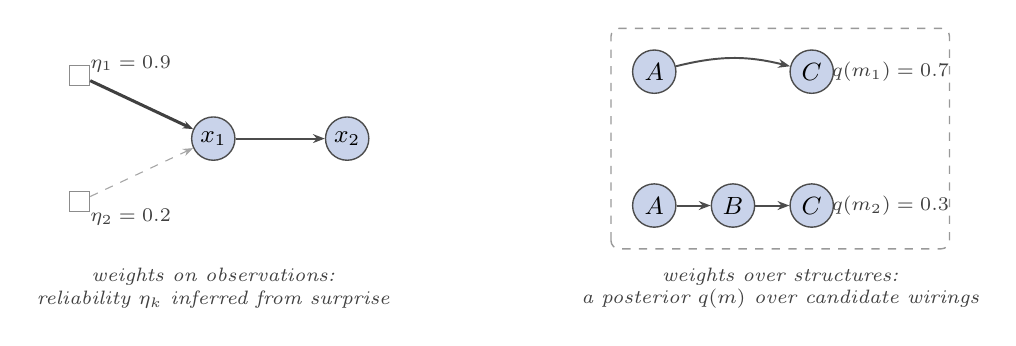
\begin{tikzpicture}[
  nd/.style={circle,draw=black!70,line width=0.5pt,fill=costc!25,minimum size=5.5mm,inner sep=0pt,font=\small},
  dep/.style={-{Stealth[length=1.5mm]},line width=0.7pt,black!70},
  wlab/.style={font=\scriptsize,text=black!75}]
  % ---- left: weights on observations ----
  \node[nd] (X1) at (0,0) {$x_1$};
  \node[nd] (X2) at (1.7,0) {$x_2$};
  \draw[dep] (X1)--(X2);
  \node[obs] (O1) at (-1.7,0.8) {};
  \node[obs] (O2) at (-1.7,-0.8) {};
  \draw[-{Stealth[length=1.3mm]},line width=1.1pt,black!75] (O1)--(X1);
  \draw[-{Stealth[length=1.3mm]},line width=0.4pt,black!35,dashed] (O2)--(X1);
  \node[wlab] at (-1.05,0.95) {$\eta_1=0.9$};
  \node[wlab] at (-1.05,-1.0) {$\eta_2=0.2$};
  \node[anno,align=center] at (0,-1.9) {weights on observations:\\reliability $\eta_k$ inferred from surprise};
  % ---- right: weights over structures ----
  \begin{scope}[shift={(5.6,0)}]
    \node[nd] (A1) at (0,0.85) {$A$};
    \node[nd] (C1) at (2.0,0.85) {$C$};
    \draw[dep] (A1) to[bend left=14] (C1);
    \node[nd] (A2) at (0,-0.85) {$A$};
    \node[nd] (B2) at (1.0,-0.85) {$B$};
    \node[nd] (C2) at (2.0,-0.85) {$C$};
    \draw[dep] (A2)--(B2); \draw[dep] (B2)--(C2);
    \node[wlab] at (3.0,0.85) {$q(m_1)=0.7$};
    \node[wlab] at (3.0,-0.85) {$q(m_2)=0.3$};
    \draw[black!40,dashed,line width=0.5pt,rounded corners=3pt] (-0.55,-1.4) rectangle (3.75,1.4);
    \node[anno,align=center] at (1.6,-1.9) {weights over structures:\\a posterior $q(m)$ over candidate wirings};
  \end{scope}
\end{tikzpicture}}
\caption{Representing diversity. \emph{Left:} each observation channel carries an inferred
reliability weight $\eta_k$ (Eq.~\ref{eq:lambda})---a hyperprior through which trust is
learned rather than fixed. \emph{Right:} the same move one level up: an agent holds two
candidate structures---$A\!\to\!C$ direct versus $A\!\to\!B\!\to\!C$---with a posterior
$q(m)$ over them, so different readings of the same evidence are held apart rather than
averaged.}
\label{fig:diversity}
\end{figure}

\emph{Weights on observations.} Stop treating a channel's precision as a constant and
\emph{infer} it \citep{ohagan2012}: carried as a scale mixture, each
channel's noise precision becomes a latent with its own prior, and its posterior expectation,
given the standardized one-step surprise $z_k^2$ (the squared residual of observation $k$
against the agent's own prediction, in units of its predictive variance), is the classic
Student-$t$ weight
\begin{equation}
\eta_k \;=\; \frac{\nu+1}{\nu+z_k^2},
\label{eq:lambda}
\end{equation}
applied multiplicatively to the channel's evidence deposit: \emph{trust what does not keep
surprising you}. The single dial $\nu$ sets how quickly surprise becomes doubt, and
$\nu\to\infty$ recovers the Gaussian defaults exactly. Pointed \emph{between} agents, the
same functional is precision learning at the social level,
$\eta_{ij}=(\nu_s+1)/(\nu_s+z_{ij}^2)$ on the calibrated disagreement between $i$ and
$j$---readable from \emph{opinions} or from \emph{wiring}, the contested coupling entries of
$\Pi$ (Appendix~\ref{app:reliability}). These weights add no objective and no memory, stay
strictly positive, and default to off, reproducing the baseline byte-identically.

\emph{Weights over structures.}\label{sec:rivals}
This is where the diversity claim lives. Inferred reliability says how much to trust a
source; it cannot represent the \emph{alternative} a source argues for. So each agent carries
$K$ candidate wirings $(\Pi_k,h_k)$ and a posterior over a model index---$q_i(x,m)$ rather
than $q_i(x)$---each candidate scored every step by its prequential predictive density
\emph{before} the shared deposit lands, so structure-discriminating evidence accumulates in
the log-weights $L_{ik}$ instead of being erased. Communication changes accordingly:
parameter beliefs fuse only \emph{within} a frame (candidate $k$ with neighbours' candidate
$k$, never averaged across frames), and what travels between frames is the hypothesis itself,
by damped log-linear pooling of the log-weights, $L\leftarrow(1-\alpha_m)L+\alpha_m W L$. The
damping gives the pooled log-odds a fixed point at a constant gap set by each camp's own
evidence (${\sim}\,s/2\alpha_m$ nats for two symmetric camps), where reliability weights
alone leave consensus as the only fixed point. $K=1$ reduces exactly to the baseline's
fuse-then-observe, so the comparisons of \S\ref{sec:results} run all three architectures on
byte-identical observation streams (Appendix~\ref{app:reliability}).

% ======================================================================
\subsection{The simulation at a glance}
\label{sec:model}
% ======================================================================

The sweep of Appendix~\ref{app:null} instantiates the phlogiston world: a hub-structured
paradigm net in which one core commitment is load-bearing for combustion, calcination and
respiration; at a fixed step the world flips (the calx is heavier---the gravimetric anomaly),
and the truth thereafter contains a dimension (oxygen) in \emph{no agent's network}. One round
of the simulation, for every agent:

\begin{enumerate}\itemsep1pt
\item \textbf{Observe.} The world emits observations at the belt; disconfirming channels carry
the conviction-gate weight $w_k$ (\S\ref{sec:revision}) and, with the reliability gate on, the
inferred $\eta_k$ (Eq.~\ref{eq:lambda}).
\item \textbf{Infer.} Exact linear-Gaussian update of the value-tilted posterior
(Eq.~\ref{eq:tilted}); precision accumulates.
\item \textbf{Crisis check (reduction).} Candidate prunes are scored by
$\Delta F+\lambda_i\,\Delta U$, both terms closed-form from the Savage--Dickey reduced
posterior (Eq.~\ref{eq:bmr}); both protective belt edges clearing the bar is a \emph{crisis},
and the hub is released (Appendix~\ref{app:crisis-discovery}).
\item \textbf{Fuse.} Posteriors and structural edits pool across the trust graph, weighted by
the intra/inter coupling and, with the social gate on, by $\eta_{ij}$
(\S\ref{sec:reliability}); pooling all dimensions vs.\ only those jointly represented is a
protocol choice with consequences (Appendix~\ref{app:null}).
\item \textbf{Forget.} Accumulated precision decays by $\omega$ (\S\ref{sec:temporal}).
\end{enumerate}

Crisis and reduction are thus not stipulated events but threshold crossings of the model's own
evidence; Appendix~\ref{app:crisis-discovery} derives the check from the single tilted
objective and lists explicitly what remains a modelling commitment. Note what the loop does
\emph{not} contain: an expansion step. By the scope choice of \S\ref{sec:structurelearning},
the model only ever prunes; novelty in the main text is supplied, never conceived, and only
the earlier phlogiston prototype reported in Appendix~\ref{app:null} runs the full cycle
with a Poisson-arrival expansion check.
Table~\ref{tab:dials} (Appendix~\ref{app:null}) lists the dials swept; everything else is held
fixed, and all code is seeded and ships its own null and positive controls.

One thing deserves emphasis before the results: every baseline ingredient above is its field's
default---Kalman-filter belief updating, the standard formalization of motivated reasoning,
classical opinion pooling in information form, textbook Bayesian model comparison. Nothing
exotic has been smuggled in; the results test what these defaults can do \emph{together}.

% ======================================================================
\section{Results}
\label{sec:results}
% ======================================================================

All results are from the population of \S\ref{sec:carryover}, run by the loop of
\S\ref{sec:model}; the full Kuhnian-cycle sweep on the phlogiston world is summarized, with
the simulation described, in Appendix~\ref{app:null}, and experiment details are in
Appendix~\ref{app:reliability}. The nets are hand-wired to expose the geometry, not fitted to
data.

\subsection{Averaging collapses structural diversity; represented rivals hold it}
\label{sec:res-homogeneity}
\label{sec:res-distinct}

The baseline behaviour follows from the fusion step itself. Fusion is precision-weighted
averaging on a connected trust graph---DeGroot dynamics in information form
\citep{degroot1974,acemoglu2011}---and opinion dynamics has long known what such pooling
does: it is a contraction, so disagreement decays geometrically toward consensus, and a
Gaussian agent never rejects a conflicting source---it averages it in
\citep{dawid1973,ohagan1979,ohagan2012}. Active inference has begun to ask the same question
of its own fusion step---whether belief sharing is a blessing or a curse
\citep{catal2024}---and over structured Bayes nets the answer has a one-line algebraic face:
$|\,\mathrm{mean}_i\,\Pi_i\,|\le\max_i|\Pi_i|$ entrywise, so an
average can never \emph{create} an edge absent from every individual---whatever a collective
knows beyond its members lives in the \emph{union} of their networks, never in their
average.

The experiment: two camps in full contact on a shared world, each running only its own
commitment's experiment---theory-laden evidence, the Kuhnian condition---and three
architectures on byte-identical observation streams: plain fusion (the default), the
Student-$t$ trust weights of \S\ref{sec:reliability}, and the structure posterior of
\S\ref{sec:rivals}. We measure the inter-camp \emph{structure distance} $D(t)$: small when
the camps wire the world the same way, large when they hold different wirings.

Figure~\ref{fig:res-walls} is the result. Under plain fusion the inter-camp distance
collapses within a few steps: the contraction. Under the trust weights the gap holds for
hundreds of steps, then visibly decays---the weights are memoryless and stay strictly
positive, so consensus remains the only fixed point; what they buy, they buy as time. (What
the weights \emph{read} also decides: pointed at opinions they never fire, because both camps
fit the same blended data and agree in their means; pointed at the wiring they retain $94\%$
of the divergence where fixed trust keeps $10\%$---Appendix~\ref{app:reliability}.) With represented rivals---$K$ candidate wirings and a
posterior over them, so each camp can see the difference between the models---the gap stays
flat to $t=1500$, each camp internally certain of its own theory: a fixed point of the damped
hypothesis-pooling dynamics, not a slow leak (Appendix~\ref{app:reliability}).

\begin{figure}[h!]
\centering
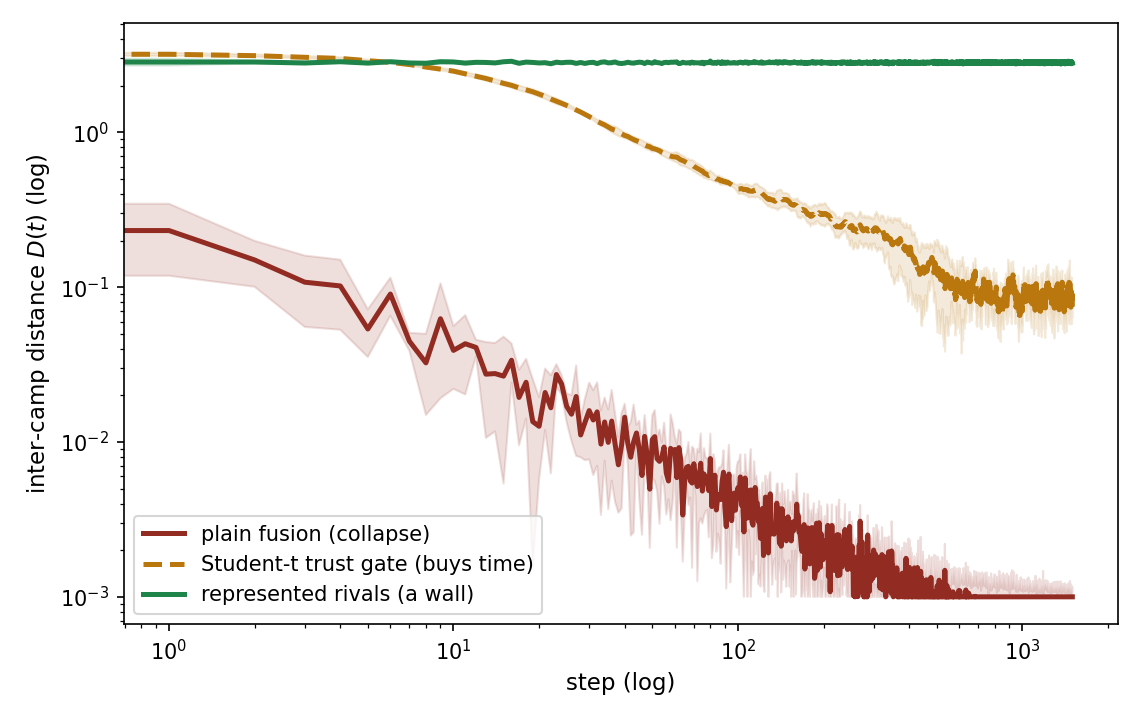
\includegraphics[width=0.62\linewidth]{fig_walls_vs_time.png}
\caption{Same setups, same evidence---only the representation differs (two camps, full
contact, theory-laden streams; inter-camp distance $D(t)$, mean $\pm$ s.d., 5 seeds, log--log).
Plain fusion collapses (the contraction); the Student-$t$ gate decays (time, bought and spent);
represented rivals hold. Each architecture runs its own best memory setting
(Appendix~\ref{app:reliability}).}
\label{fig:res-walls}
\end{figure}

\subsection{The Kuhn cycle with represented rivals: crisis as a state}
\label{sec:res-kuhn}

With the structure posterior in place, the Kuhnian transition itself can be run
(Fig.~\ref{fig:res-kuhncycle}). A population holds two candidate wirings of the phlogiston
world---the incumbent and the oxygen reading---and the world turns at the dotted line. Normal
science forms endogenously: from a uniform start, the population commits to the incumbent and
$q(\mathrm{oxygen})$ sits at zero. After the world turns, the model posterior goes
\emph{torn}: the entropy of $q(m)$ rises to a peak while $q(\mathrm{oxygen})$ climbs---crisis
as a \emph{state} of the belief, not a stipulated event---and then resolves as the population
flips to the new paradigm and recommits: revolution, then a new normal. In the Gaussian
baseline none of these phases exists: there is no $q(m)$ to go torn, and the transition is
invisible from the belief state.

\begin{figure}[h!]
\centering
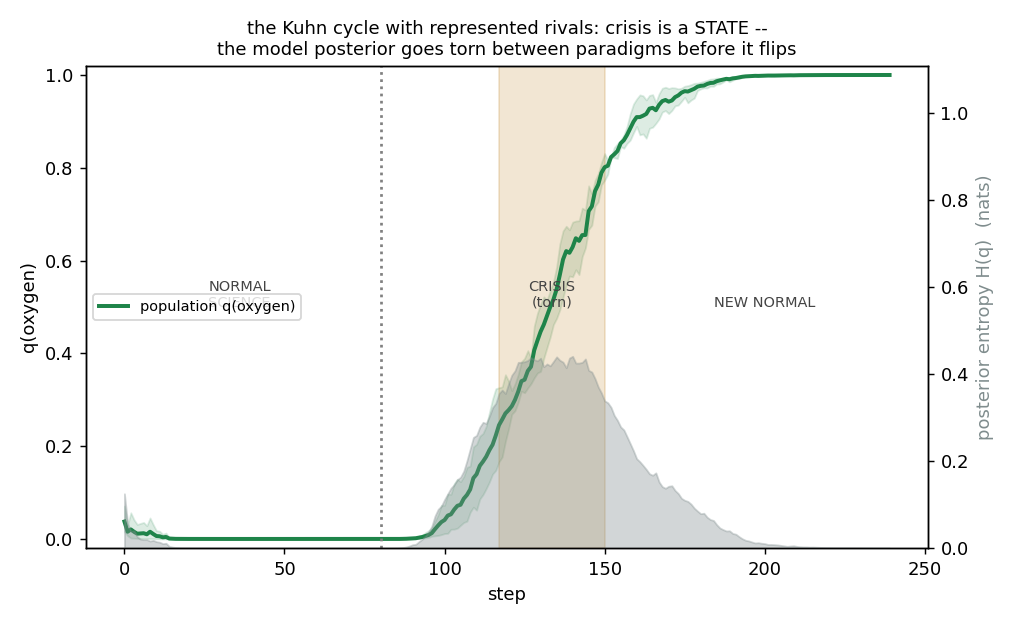
\includegraphics[width=0.8\linewidth]{fig_rival_kuhn_cycle.png}
\caption{The Kuhn cycle with represented rivals (population mean $\pm$ s.d.; the world turns
at the dotted line). Green: the population posterior on the oxygen reading,
$q(\mathrm{oxygen})$. Grey: the entropy of the model posterior $H(q(m))$, peaking in the
shaded band---crisis as a torn state between paradigms---before the flip completes. Normal
science, crisis, revolution, new normal, all read off one belief state.}
\label{fig:res-kuhncycle}
\end{figure}

Boundaries, stated plainly. The demonstrations are deliberately small---one agent, $N=60$,
then $N=16$, on hand-wired worlds---existence proofs that the persistence was representational, not
sweeps of social topologies (the one such sweep---this transition replayed across four
reference contact graphs---is in Appendix~\ref{app:reliability}). No model expansion runs anywhere in the main text
(\S\ref{sec:structurelearning}): the rival mechanism is \emph{given} its $K$ candidates, and
anchored forgetting on the candidate nets is part of the mechanism---keeping a rival
represented means not letting accumulated evidence drown it. What it does not yet do is named:
under log-linear pooling a lone discoverer's candidate is majority-swamped, and no agent yet
\emph{acts} on where its candidates disagree---the crucial experiment. Controls: a world that
never shifts produces no doubt; gates and rivals off reproduce the baseline
byte-identically; no bar is tuned (Appendix~\ref{app:reliability}).

% ======================================================================
\section{Discussion}
\label{sec:discussion}
% ======================================================================

Taken together, the results return us to the opening premise. Communities of reasoning
agents---scientific ones, and increasingly the artificial ones built around them---are asked
to be \emph{open-ended}: to keep representing new structure, not merely to refine the
structure they already share. The results say what that requires. When each agent's paradigm
is a single Gaussian belief net and combination is precision-weighted averaging, divergence
does not survive contact: the community converges on a compromise network no member holds,
however the dials are set (Result 1). When agents can instead hold different structures
apart---candidate wirings with a posterior over them, hypotheses communicated rather than
averaged---divergence survives full contact (Result 2). Stated as one finding: a community
doing Bayesian model reduction over structured Bayes nets needs the ability to represent the
\emph{difference between models} inside each agent. Without that ability there is no
divergence; without divergence, no open-endedness.

The homogenization is thus a failure of \emph{representation}, not of tuning. There is no
coordinate in $(\Pi,h)$ whose value can mean \emph{torn between two hypotheses}: conflict
arrives as growing confidence, and fusion erases who disagreed about what---which is why no
dial of the sweep escaped it, and why inferred reliability could only slow it. The structure
posterior of \S\ref{sec:rivals} is that diagnosis made executable: multiple structural
hypotheses per agent (an agent that can be torn), divergence between live candidates as a
computable state, and communication of hypotheses---fusion within frames, never averaging
across them.

The relation to Kuhn is now allegory-free: the regime \emph{holds} normal science (the derived
core and belt of \S\ref{sec:carryover}).
Of the revolutionary remainder, inferred reliability \emph{supplies} crisis as suspended
confidence and renders incommensurability \citep{kuhn1983} a timescale, while represented
rivals make it a \emph{state}: two camps internally certain of different wirings at a fixed
point, the gestalt switch given its slot (a $q(m)$ that flips on prequential evidence). And
any community whose aggregation step averages rather than gates inherits the regime's
signature, whatever the sophistication of its members---the same sharing that lets a group
synchronise its members' anticipations and act as one \citep{albarracin2024protentions} is
what averages the dissenter away: a population of structure learners is
only as open-ended as its pooling permits---and as what its pooling \emph{reads}
(\S\ref{sec:res-distinct})---a property of the protocol, designed in rather than an emergent
grace of scale.

\paragraph{Limitations and future work.}
The demonstrations are small and the nets hand-wired; the claims are existence proofs about
representation, not sweeps of social topologies. The clearest next step is the expansion this
paper deferred (\S\ref{sec:structurelearning})---and the structure posterior suggests where
to point it. The divergence between an agent's live candidates is a computable map: the KL
divergence between the predictive distributions their couplings induce, the same functional
Bayesian model reduction already scores prunes with (Eq.~\ref{eq:bmr}). Read forward instead
of backward, that map is a natural \emph{prior over where to expand}: new structure is most
likely to pay exactly where the represented models disagree. Beyond this---and the swamped
discoverer and unchosen crucial experiment already named in \S\ref{sec:res-distinct}---lies the
deepest exit: a new \emph{instrument} enlarges the likelihood's own support, and one cannot
place a posterior over the unconceived \citep{stanford2006}. What a community controls is how
hard it looks---and, above all, what its pooling does to the member who finds it first.

% ======================================================================
\begin{thebibliography}{99}

\bibitem[Albarracin et al.(2022)]{albarracin2022}
M.~Albarracin, D.~Demekas, M.~J.~D.~Ramstead, and C.~Heins.
Epistemic communities under active inference. \emph{Entropy}, 24(4):476, 2022.

\bibitem[\c{C}atal et al.(2024)]{catal2024}
O.~\c{C}atal, T.~Van~de~Maele, R.~J.~Pitliya, M.~Albarracin, C.~Pattisapu, and T.~Verbelen.
Belief sharing: a blessing or a curse. arXiv:2407.02465, 2024.

\bibitem[Dalege et al.(2016)]{dalege2016}
J.~Dalege, D.~Borsboom, F.~van Harreveld, H.~van den Berg, M.~Conner, and H.~L.~J.~van der Maas.
Toward a formalized account of attitudes: the Causal Attitude Network (CAN) model.
\emph{Psychological Review}, 123(1):2--22, 2016.

\bibitem[Dawid(1973)]{dawid1973}
A.~P.~Dawid.
Posterior expectations for large observations. \emph{Biometrika}, 60(3):664--667, 1973.

\bibitem[O'Hagan(1979)]{ohagan1979}
A.~O'Hagan.
On outlier rejection phenomena in Bayes inference.
\emph{Journal of the Royal Statistical Society, Series B}, 41(3):358--367, 1979.

\bibitem[O'Hagan and Pericchi(2012)]{ohagan2012}
A.~O'Hagan and L.~Pericchi.
Bayesian heavy-tailed models and conflict resolution: a review.
\emph{Brazilian Journal of Probability and Statistics}, 26(4):372--401, 2012.

\bibitem[Friedman et al.(2008)]{friedman2008glasso}
J.~Friedman, T.~Hastie, and R.~Tibshirani.
Sparse inverse covariance estimation with the graphical lasso.
\emph{Biostatistics}, 9(3):432--441, 2008.

\bibitem[Friston and Penny(2011)]{friston2011}
K.~J.~Friston and W.~Penny.
Post hoc Bayesian model selection. \emph{NeuroImage}, 56(4):2089--2099, 2011.

\bibitem[Friston et al.(2015)]{friston2015}
K.~Friston, F.~Rigoli, D.~Ognibene, C.~Mathys, T.~Fitzgerald, and G.~Pezzulo.
Active inference and epistemic value. \emph{Cognitive Neuroscience}, 6(4):187--214, 2015.

\bibitem[Friston et al.(2017)]{friston2017curiosity}
K.~J.~Friston, M.~Lin, C.~D.~Frith, G.~Pezzulo, J.~A.~Hobson, and S.~Ondobaka.
Active inference, curiosity and insight. \emph{Neural Computation}, 29(10):2633--2683, 2017.

\bibitem[Friston et al.(2018)]{friston2018bmr}
K.~J.~Friston, T.~Parr, and P.~Zeidman.
Bayesian model reduction. arXiv:1805.07092, 2018.

\bibitem[Hawkes(1971)]{hawkes1971}
A.~G.~Hawkes.
Spectra of some self-exciting and mutually exciting point processes.
\emph{Biometrika}, 58(1):83--90, 1971.

\bibitem[Hohwy(2016)]{hohwy2016}
J.~Hohwy.
The self-evidencing brain. \emph{No\^us}, 50(2):259--285, 2016.

\bibitem[Hughes et al.(2024)]{hughes2024}
E.~Hughes, M.~Dennis, J.~Parker-Holder, F.~Behbahani, A.~Mavalankar, Y.~Shi, T.~Schaul, and
T.~Rockt\"aschel.
Position: open-endedness is essential for artificial superhuman intelligence.
In \emph{Proceedings of the 41st International Conference on Machine Learning}, PMLR 235, 2024.

\bibitem[Hyland and Albarracin(2025)]{hyland2025}
D.~Hyland and M.~Albarracin.
On the variational costs of changing our minds. arXiv:2509.17957, 2025.
(Also in \emph{Active Inference: IWAI 2025}, CCIS vol.~2857, Springer, 2026,
doi:10.1007/978-3-032-16955-6\_1.)

\bibitem[Jonard et al.(2025)]{jonard2025}
N.~Jonard, S.~Reijula, and L.~Marengo.
Theory choice in epistemic networks: five ways to avoid premature convergence. PhilSci Archive, 2025.

\bibitem[Kitcher(1990)]{kitcher1990}
P.~Kitcher.
The division of cognitive labor. \emph{Journal of Philosophy}, 87(1):5--22, 1990.

\bibitem[Koller and Friedman(2009)]{koller2009}
D.~Koller and N.~Friedman.
\emph{Probabilistic Graphical Models: Principles and Techniques}. MIT Press, 2009.

\bibitem[Kuhn(1962)]{kuhn1962}
T.~S.~Kuhn.
\emph{The Structure of Scientific Revolutions}. University of Chicago Press, 1962.

\bibitem[MacKay(1992)]{mackay1992}
D.~J.~C.~MacKay.
Bayesian interpolation. \emph{Neural Computation}, 4(3):415--447, 1992.

\bibitem[Millidge et al.(2021)]{millidge2021}
B.~Millidge, A.~Tschantz, and C.~L.~Buckley.
Whence the expected free energy? \emph{Neural Computation}, 33(2):447--482, 2021.

\bibitem[Neal(1996)]{neal1996}
R.~M.~Neal.
\emph{Bayesian Learning for Neural Networks}.
Lecture Notes in Statistics 118, Springer, 1996.

\bibitem[Nguyen(2020)]{nguyen2018}
C.~T.~Nguyen.
Echo chambers and epistemic bubbles. \emph{Episteme}, 17(2):141--161, 2020.

\bibitem[O'Connor and Weatherall(2019)]{oconnor2019}
C.~O'Connor and J.~O.~Weatherall.
\emph{The Misinformation Age}. Yale University Press, 2019.

\bibitem[Parr and Friston(2017)]{parr2017uncertainty}
T.~Parr and K.~J.~Friston.
Uncertainty, epistemics and active inference.
\emph{Journal of the Royal Society Interface}, 14(136):20170376, 2017.

\bibitem[Smith et al.(2020)]{smith2020structure}
R.~Smith, P.~Schwartenbeck, T.~Parr, and K.~J.~Friston.
An active inference approach to modeling structure learning: concept learning as an example case.
\emph{Frontiers in Computational Neuroscience}, 14:41, 2020.

\bibitem[Stanford(2006)]{stanford2006}
P.~K.~Stanford.
\emph{Exceeding Our Grasp: Science, History, and the Problem of Unconceived Alternatives}.
Oxford University Press, 2006.

\bibitem[Stanley et al.(2017)]{stanley2017oe}
K.~O.~Stanley, J.~Lehman, and L.~Soros.
Open-endedness: the last grand challenge you've never heard of. \emph{O'Reilly Radar}, 2017.

\bibitem[Strevens(2003)]{strevens2003}
M.~Strevens.
The role of the priority rule in science. \emph{Journal of Philosophy}, 100(2):55--79, 2003.

\bibitem[Thagard(1989)]{thagard1989}
P.~Thagard.
Explanatory coherence. \emph{Behavioral and Brain Sciences}, 12(3):435--467, 1989.

\bibitem[Tipping(2001)]{tipping2001}
M.~E.~Tipping.
Sparse Bayesian learning and the relevance vector machine.
\emph{Journal of Machine Learning Research}, 1:211--244, 2001.

\bibitem[Zollman(2010)]{zollman2010}
K.~J.~S.~Zollman.
The epistemic benefit of transient diversity. \emph{Erkenntnis}, 72(1):17--35, 2010.

\bibitem[Griffiths and Ghahramani(2011)]{griffiths2011ibp}
T.~L.~Griffiths and Z.~Ghahramani.
The Indian Buffet Process: an introduction and review.
\emph{Journal of Machine Learning Research}, 12:1185--1224, 2011.

\bibitem[Kemp and Tenenbaum(2008)]{kemp2008form}
C.~Kemp and J.~B.~Tenenbaum.
The discovery of structural form.
\emph{Proceedings of the National Academy of Sciences}, 105(31):10687--10692, 2008.

\bibitem[Ullman et al.(2012)]{ullman2012}
T.~D.~Ullman, N.~D.~Goodman, and J.~B.~Tenenbaum.
Theory learning as stochastic search in a language of thought.
\emph{Cognitive Development}, 27(4):455--480, 2012.

\bibitem[Friston et al.(2017b)]{friston2017process}
K.~Friston, T.~FitzGerald, F.~Rigoli, P.~Schwartenbeck, and G.~Pezzulo.
Active inference: a process theory. \emph{Neural Computation}, 29(1):1--49, 2017.

\bibitem[Mathys et al.(2011)]{mathys2011}
C.~Mathys, J.~Daunizeau, K.~J.~Friston, and K.~E.~Stephan.
A Bayesian foundation for individual learning under uncertainty.
\emph{Frontiers in Human Neuroscience}, 5:39, 2011.

\bibitem[Smith et al.(2022)]{smith2022tutorial}
R.~Smith, K.~J.~Friston, and C.~Whyte.
A step-by-step tutorial on active inference and its application to empirical data.
\emph{Journal of Mathematical Psychology}, 107:102632, 2022.

\bibitem[Da Costa et al.(2020)]{dacosta2020}
L.~Da Costa, T.~Parr, N.~Sajid, S.~Veselic, V.~Neacsu, and K.~Friston.
Active inference on discrete state-spaces: a synthesis.
\emph{Journal of Mathematical Psychology}, 99:102447, 2020.

\bibitem[Holmes(2000)]{holmes2000}
F.~L.~Holmes.
The revolution in chemistry and physics: overthrow of a reigning paradigm or competition between
contemporary research programs? \emph{Isis}, 91(4):735--753, 2000.

\bibitem[Thagard(1990)]{thagard1990}
P.~Thagard.
The conceptual structure of the chemical revolution.
\emph{Philosophy of Science}, 57(2):183--209, 1990.

\bibitem[Boantza and Gal(2011)]{boantza2011}
V.~D.~Boantza and O.~Gal.
The `absolute existence' of phlogiston: the losing party's point of view.
\emph{British Journal for the History of Science}, 44(3):317--342, 2011.

\bibitem[Blumenthal and Ladyman(2017)]{blumenthal2017}
G.~Blumenthal and J.~Ladyman.
The development of problems within the phlogiston theories, 1766--1791.
\emph{Foundations of Chemistry}, 19(3):241--280, 2017.

\bibitem[Ball et al.(2024)]{polygraphs2024}
B.~Ball, A.~Koliousis, A.~Mohanan, and M.~Peacey.
Computational philosophy: reflections on the {PolyGraphs} project.
\emph{Humanities and Social Sciences Communications}, 11:186, 2024.

\bibitem[Michelini et al.(2023)]{michelini2023}
M.~Michelini, J.~Osorio, W.~Houkes, D.~\v{S}e\v{s}elja, and C.~Stra\ss{}er.
Scientific disagreements and the diagnosticity of evidence: how too much data may lead to polarization.
\emph{Journal of Artificial Societies and Social Simulation}, 26(4):5, 2023.

\bibitem[Albarracin et al.(2024)]{albarracin2024protentions}
M.~Albarracin, R.~J.~Pitliya, T.~St.~Clere Smithe, D.~A.~Friedman, K.~Friston, and M.~J.~D.~Ramstead.
Shared protentions in multi-agent active inference.
\emph{Entropy}, 26(4):303, 2024.

\bibitem[Friston et al.(2024a)]{friston2023federated}
K.~J.~Friston, T.~Parr, C.~Heins, A.~Constant, D.~Friedman, T.~Isomura, C.~Fields,
T.~Verbelen, M.~Ramstead, J.~Clippinger, and C.~D.~Frith.
Federated inference and belief sharing.
\emph{Neuroscience \& Biobehavioral Reviews}, 156:105500, 2024.

\bibitem[Waade et al.(2025)]{waade2025}
P.~T.~Waade, C.~L.~Olesen, J.~E.~Laursen, S.~W.~Nehrer, C.~Heins, K.~Friston, and C.~Mathys.
As one and many: relating individual and emergent group-level generative models in active inference.
\emph{Entropy}, 27(2):143, 2025.

\bibitem[Ullman and Tenenbaum(2020)]{ullman2020}
T.~D.~Ullman and J.~B.~Tenenbaum.
Bayesian models of conceptual development: learning as building models of the world.
\emph{Annual Review of Developmental Psychology}, 2:533--558, 2020.

\bibitem[Neacsu et al.(2022)]{neacsu2022}
V.~Neacsu, M.~B.~Mirza, R.~A.~Adams, and K.~J.~Friston.
Structure learning enhances concept formation in synthetic active inference agents.
\emph{PLOS ONE}, 17(11):e0277199, 2022.

\bibitem[Priorelli and Stoianov(2023)]{priorelli2023}
M.~Priorelli and I.~P.~Stoianov.
Dynamic inference by model reduction.
\emph{bioRxiv}, 2023. doi:10.1101/2023.09.10.557043.

\bibitem[Friston et al.(2016)]{friston2016peb}
K.~J.~Friston, V.~Litvak, A.~Oswal, A.~Razi, K.~E.~Stephan, B.~C.~M.~van Wijk, G.~Ziegler, and
P.~Zeidman. Bayesian model reduction and empirical {Bayes} for group ({DCM}) studies.
\emph{NeuroImage}, 128:413--431, 2016.

\bibitem[Friston et al.(2024b)]{friston2024ci}
K.~J.~Friston et al.
Designing ecosystems of intelligence from first principles.
\emph{Collective Intelligence}, 3(4), 2024. arXiv:2212.01354.

\bibitem[Kaufmann et al.(2021)]{kaufmann2021}
R.~Kaufmann, P.~Gupta, and J.~Taylor.
An active inference model of collective intelligence.
\emph{Entropy}, 23(7):830, 2021.

\bibitem[Acemoglu and Ozdaglar(2011)]{acemoglu2011}
D.~Acemoglu and A.~Ozdaglar.
Opinion dynamics and learning in social networks.
\emph{Dynamic Games and Applications}, 1(1):3--49, 2011.

\bibitem[Bala and Goyal(1998)]{balagoyal1998}
V.~Bala and S.~Goyal.
Learning from neighbours. \emph{Review of Economic Studies}, 65(3):595--621, 1998.

\bibitem[Bohren and Hauser(2021)]{bohren2021}
J.~A.~Bohren and D.~N.~Hauser.
Learning with heterogeneous misspecified models: characterization and robustness.
\emph{Econometrica}, 89(6):3025--3077, 2021.

\bibitem[Bollen(1987)]{bollen1987}
K.~A.~Bollen.
Total, direct, and indirect effects in structural equation models.
\emph{Sociological Methodology}, 17:37--69, 1987.

\bibitem[Bonacich(1987)]{bonacich1987}
P.~Bonacich.
Power and centrality: a family of measures.
\emph{American Journal of Sociology}, 92(5):1170--1182, 1987.

\bibitem[DeGroot(1974)]{degroot1974}
M.~H.~DeGroot.
Reaching a consensus. \emph{Journal of the American Statistical Association}, 69(345):118--121, 1974.

\bibitem[Feyerabend(1975)]{feyerabend1975}
P.~Feyerabend.
\emph{Against Method}. New Left Books, 1975.

\bibitem[Genest and Zidek(1986)]{genest1986}
C.~Genest and J.~V.~Zidek.
Combining probability distributions: a critique and an annotated bibliography.
\emph{Statistical Science}, 1(1):114--135, 1986.

\bibitem[Hegselmann and Krause(2002)]{hegselmann2002}
R.~Hegselmann and U.~Krause.
Opinion dynamics and bounded confidence: models, analysis and simulation.
\emph{Journal of Artificial Societies and Social Simulation}, 5(3), 2002.

\bibitem[Katz(1953)]{katz1953}
L.~Katz.
A new status index derived from sociometric analysis. \emph{Psychometrika}, 18(1):39--43, 1953.

\bibitem[Kuhn(1983)]{kuhn1983}
T.~S.~Kuhn.
Commensurability, comparability, communicability.
\emph{PSA: Proceedings of the Biennial Meeting of the Philosophy of Science Association},
1982(2):669--688, 1983.

\bibitem[Lakatos(1970)]{lakatos1970}
I.~Lakatos.
Falsification and the methodology of scientific research programmes.
In I.~Lakatos and A.~Musgrave, editors, \emph{Criticism and the Growth of Knowledge},
pages 91--196. Cambridge University Press, 1970.

\bibitem[Laudan(1977)]{laudan1977}
L.~Laudan.
\emph{Progress and Its Problems: Towards a Theory of Scientific Growth}.
University of California Press, 1977.

\bibitem[Laudan(1984)]{laudan1984}
L.~Laudan.
\emph{Science and Values: The Aims of Science and Their Role in Scientific Debate}.
University of California Press, 1984.

\bibitem[Lehrer and Wagner(1981)]{lehrer1981}
K.~Lehrer and C.~Wagner.
\emph{Rational Consensus in Science and Society}. D.~Reidel, 1981.

\bibitem[Malioutov et al.(2006)]{malioutov2006}
D.~M.~Malioutov, J.~K.~Johnson, and A.~S.~Willsky.
Walk-sums and belief propagation in Gaussian graphical models.
\emph{Journal of Machine Learning Research}, 7:2031--2064, 2006.

\bibitem[O'Connor and Weatherall(2018)]{oconnorpolar2018}
C.~O'Connor and J.~O.~Weatherall.
Scientific polarization. \emph{European Journal for Philosophy of Science}, 8(3):855--875, 2018.

\bibitem[Ortega and Braun(2013)]{ortega2013}
P.~A.~Ortega and D.~A.~Braun.
Thermodynamics as a theory of decision-making with information-processing costs.
\emph{Proceedings of the Royal Society A}, 469(2153):20120683, 2013.

\bibitem[Todorov(2009)]{todorov2009}
E.~Todorov.
Efficient computation of optimal actions.
\emph{Proceedings of the National Academy of Sciences}, 106(28):11478--11483, 2009.

\bibitem[Wright(1934)]{wright1934}
S.~Wright.
The method of path coefficients. \emph{Annals of Mathematical Statistics}, 5(3):161--215, 1934.

\bibitem[Zollman(2013)]{zollman2013}
K.~J.~S.~Zollman.
Network epistemology: communication in epistemic communities.
\emph{Philosophy Compass}, 8(1):15--27, 2013.

\end{thebibliography}

% ======================================================================
\clearpage
\appendix
% ======================================================================
\section{The operator and the tilt: the closed forms behind the two fields}
\label{app:operator}
% ======================================================================

This appendix is the closed-form backing for the paper's propagation machinery: it states
the structural equation model behind $p(x\mid G)$, why the operator $\Top=(I-A)^{-1}$ is a
finite sum, and what the value tilt of Eq.~\eqref{eq:tilted} does to the posterior, exactly.
Consult it for the algebra behind the two fields $\kappa=\Top\bone$ (Eq.~\ref{eq:kappa}) and
$U=\Top u$ (Eq.~\ref{eq:U}), for the mind-change cost the revision objective prices
(Eq.~\ref{eq:mindcost}), and for the transpose convention needed to reproduce either field
against the released code. Nothing here is required to follow the results; it is the warrant
for the main text's claim that every quantity it uses is closed form.

\paragraph{How propagation is represented.} The couplings form a structural equation model $x=Ax+\zeta$,
$\zeta\sim\mathcal N(0,D^{-1})$ with $A$ the weighted DAG adjacency \citep{koller2009}; the choice is
for tractability, and a nonlinear coupling would replace $\Top$ by a local linearization. The
propagation operator is the resolvent
\begin{equation}
\Top=(I-A)^{-1}=\sum_{k\ge 0}A^k,\qquad
\Top_{iw}=\!\!\sum_{\text{paths }i\rw w}\ \prod \pi\ =\ \pi_{i\rw w},
\label{eq:Top-full}
\end{equation}
the Neumann series finite because a DAG makes $A$ nilpotent. We realise $\Top$ on the coupling
magnitudes $|A|$ so downstream mass does not cancel when a child opposes a parent; the signed $A$
builds the precision matrix. We index $\Top$ so that $\kappa_i$ sums row $i$; under the SEM
convention the released code stores the transpose and computes the same fields as column-sums of
$\Top^{\!\top}$, so a reader reproducing $\Top\bone$ literally against the code's array must
transpose first.

\paragraph{The value tilt.} With honest posterior $p(x\mid o,G)=\mathcal N(\mu,\Sigma)$, the tilted
posterior of Eq.~\eqref{eq:tilted} is a pure mean shift,
$q_\lambda(x)=\mathcal N(\mu+\lambda\Sigma U,\,\Sigma)$, with cumulant-generating function
$Z(\lambda)=\lambda\,U^{\!\top}\!\mu+\tfrac12\lambda^2\,U^{\!\top}\!\Sigma U$. Note that gating a
channel ($\rho_k\to0$) \emph{raises} the posterior variance and hence $Z''$; lock-in lives in the
vanishing mean-update gain $\rho_k H_k\Sigma U$, not in the curvature.

The mind-change cost of Eq.~\eqref{eq:tilted} is anchored to the network prior
$p(x\mid G)=\mathcal N(\mu_0,\Pi_0^{-1})$: the revision $q_\lambda$ pays
\begin{equation}
\KL{q_\lambda}{p(x\mid G)}
=\tfrac12\,\delta^{\!\top}\Pi_0\,\delta
+\tfrac12\bigl[\operatorname{tr}(\Pi_0\Sigma)-\log\det(\Pi_0\Sigma)-d\bigr],
\label{eq:mindcost}
\end{equation}
with $\delta=\mu+\lambda\Sigma U-\mu_0$ and $d=\dim x$: the evidence-driven and value-driven
displacements are priced \emph{together}, in
the prior precision $\Pi_0$---exactly the off-diagonal mass the carry-over field $\kappa=\Top\bone$
summarizes. The smaller quantity $\KL{q_\lambda}{p(x\mid o,G)}=\tfrac12\lambda^2\,U^{\!\top}\!\Sigma U$
is the fidelity gap to the honest posterior, not the cost of changing one's mind: it would vanish
for an agent that followed the evidence exactly, however far the evidence moved it.

\begin{figure}[h!]
\centering
\begin{subfigure}{0.49\textwidth}\centering
\resizebox{0.92\linewidth}{!}{%
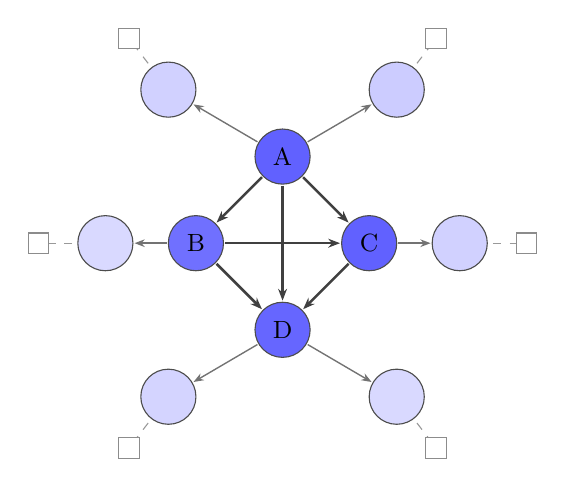
\begin{tikzpicture}
  \Positions \Edges
  \node[bel,fill=blue!62!white] at (A){A};
  \node[bel,fill=blue!56!white] at (B){B};
  \node[bel,fill=blue!62!white] at (C){C};
  \node[bel,fill=blue!60!white] at (D){D};
  \node[bel,fill=blue!18!white] at (b1){};
  \node[bel,fill=blue!20!white] at (b2){};
  \node[bel,fill=blue!15!white] at (b3){};
  \node[bel,fill=blue!18!white] at (b4){};
  \node[bel,fill=blue!17!white] at (b5){};
  \node[bel,fill=blue!15!white] at (b6){};
\end{tikzpicture}}
\par\vspace{4pt}
\resizebox{0.74\linewidth}{!}{%
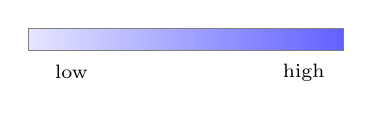
\begin{tikzpicture}
  \shade[left color=blue!10!white,right color=blue!62!white] (0,0) rectangle (4,0.28);
  \draw[black!50,line width=0.3pt] (0,0) rectangle (4,0.28);
  \node[font=\scriptsize] at (0.55,-0.28){low}; \node[font=\scriptsize] at (3.5,-0.28){high};
\end{tikzpicture}}
\caption{Revision cost $\kappa_i$ (conservatism)}
\label{sub:cost}
\end{subfigure}
\hfill
\begin{subfigure}{0.49\textwidth}\centering
\resizebox{0.92\linewidth}{!}{%
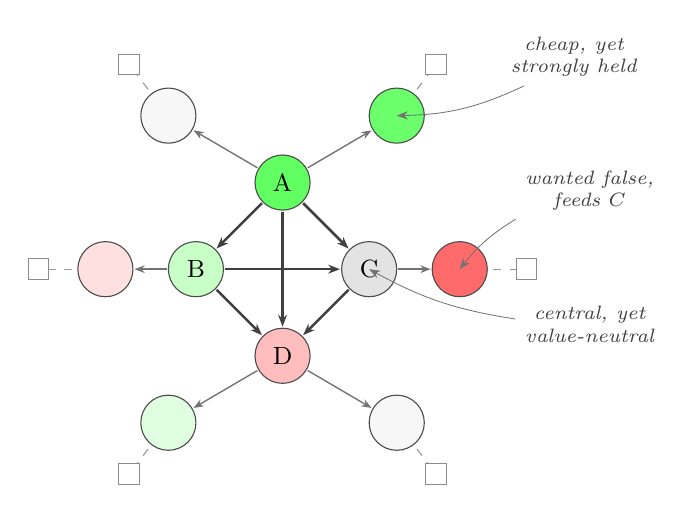
\begin{tikzpicture}
  \Positions \Edges
  \node[bel,fill=green!62!white] at (A){A};
  \node[bel,fill=green!22!white] at (B){B};
  \node[bel,fill=gray!22!white]  at (C){C};
  \node[bel,fill=red!26!white]   at (D){D};
  \node[bel,fill=gray!6!white]   at (b1){};
  \node[bel,fill=green!58!white] at (b2){};
  \node[bel,fill=red!12!white]   at (b3){};
  \node[bel,fill=red!58!white]   at (b4){};
  \node[bel,fill=green!12!white] at (b5){};
  \node[bel,fill=gray!6!white]   at (b6){};
  \node[anno] (an2) at (3.7,2.7){cheap, yet\\strongly held};
  \draw[annoarrow] (an2) to[bend left=12] (b2);
  \node[anno] (anC) at (3.9,-0.7){central, yet\\value-neutral};
  \draw[annoarrow] (anC) to[bend left=10] (C);
  \node[anno] (an4) at (3.9,1.0){wanted false,\\feeds $C$};
  \draw[annoarrow] (an4) to[bend right=10] (b4);
\end{tikzpicture}}
\par\vspace{4pt}
\resizebox{0.88\linewidth}{!}{%
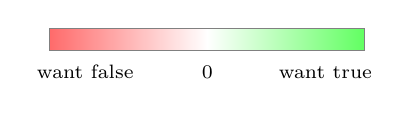
\begin{tikzpicture}
  \shade[left color=red!58!white,right color=white] (0,0) rectangle (2,0.28);
  \shade[left color=white,right color=green!62!white] (2,0) rectangle (4,0.28);
  \draw[black!50,line width=0.3pt] (0,0) rectangle (4,0.28);
  \node[font=\scriptsize] at (0.45,-0.28){want false}; \node[font=\scriptsize] at (2,-0.28){0};
  \node[font=\scriptsize] at (3.5,-0.28){want true};
\end{tikzpicture}}
\caption{Intrinsic utility $u_i$ (conviction)}
\label{sub:util}
\end{subfigure}
\caption{Two fields on one paradigm (schematic). Both panels carry the \emph{same} network---a densely
coupled core $\{A,B,C,D\}$ and a sparse belt $\{b_1,\dots,b_6\}$ in contact with observation.
\subref{sub:cost}~Revision cost is the carry-over of mind-change, $\kappa=\Top\bone$
(Eq.~\ref{eq:kappa}): a node's cost is the precision-weighted mass of its descendants, a clean radial
gradient monotone in centrality. \subref{sub:util}~Intrinsic utility is signed---beliefs one wants
true (green), wants false (red), or is neutral toward (white)---and the conviction field
$U=\Top u$ does not align with $\kappa$: $C$ is central yet value-neutral; $b_2$ is cheap yet strongly
held; $b_4$, which feeds $C$, is a conclusion the community wants false. The two fields are
$\Top\bone$ and $\Top u$, the same operator on two sources, and they are independent vectors.}
\label{fig:twofields}
\end{figure}

% ======================================================================
\section{The null regime, measured}
\label{app:null}
% ======================================================================

This appendix does two jobs for \S\ref{sec:res-homogeneity}. First, it describes the
simulation the main text only sketches: the phlogiston world---the paradigm network the
paper's experiments instantiate---and the per-round community loop as actually run in the
released experiments, in the paper's own notation. Second, it preserves, clearly flagged as
such, the headline numbers the main text still cites from an \emph{earlier and larger
prototype} of the same world: a full Kuhnian cycle with a Poisson-arrival expansion step
(Appendix~\ref{app:crisis-discovery}) and four closed-loop escape mechanisms, none of which
the model of this paper contains (\S\ref{sec:structurelearning}). Read it after Result 1,
when you want to know exactly what was run and where each quoted number comes from.

\paragraph{The phlogiston world.}
Ten named commitments form the shared basis of every net: the hidden hub
(\emph{phlogiston}), eight surface commitments it explains---combustion and calcination as
release, the metal as calx-plus-phlogiston, the sign of the mass change, gas consumption,
the air's finite capacity, reduction with charcoal, respiration as slow combustion---and the
anomaly node, \emph{the calx is heavier than the metal}. The incumbent paradigm is a
common-cause DAG: the hub is a parent of the eight surface commitments (which is what makes
the phenomena co-vary), a belt mass-balance edge makes the anomaly a child of the two
mass-law nodes, and the prior means get the anomaly \emph{wrong}---phlogiston escapes, so
the calx should be lighter. The rival paradigm drops the hub couplings entirely and keeps
the belt mass law with the \emph{correct} means: exactly the direct couplings that
marginalizing a hub leaves behind (the Schur residue,
Appendix~\ref{app:crisis-discovery}). The world flips at a fixed step
$t_{\text{shift}}$---the calx really is heavier thereafter. Observation is the gravimetric
operator $H$: one direct row per measured commitment (the level signal) plus a single
relational mass-balance row reading calx $-$ mass-change $-$ gas, the only row whose Fisher
deposit $H^{\!\top}\!\operatorname{diag}(w)\,H/\sigma_o^2$ carries off-diagonal
information---the row that can move structure.

\paragraph{The community and the round.}
The released experiments run the loop of \S\ref{sec:model} in its represented-rival
configuration (\S\ref{sec:rivals}; definitions in Appendix~\ref{app:reliability}): $N$
agents on a contact graph, each carrying the $K$ candidate wirings above ($K{=}2$,
incumbent versus rival; a $K{=}3$ ladder adds the \emph{articulated} incumbent---hub kept,
mass means patched). Per round: hypotheses pool,
$L\leftarrow(1-\alpha_m)L+\alpha_m WL$; parameter beliefs fuse within frames; every
candidate is scored by its prequential predictive density before the shared deposit lands;
the deposit lands in every candidate; anchored forgetting relaxes each candidate toward its
own prior at rate $\omega$. ($K{=}1$ is exactly the fuse-then-observe baseline---the null
regime itself.) Theory-ladenness enters as attention: a conservative community carries
weight $1-\gamma$ on the disagreement and mass-balance rows, where $\gamma$ is precisely
the silenced disconfirming fraction of Eq.~\eqref{eq:gamma}---dialled directly here rather
than derived from the conviction field through $w_k=\exp(-g|U\!\cdot\!H_k|)$ as in
\S\ref{sec:revision}---while a vanguard that keeps running the gravimetric experiment
retains full attention. Runs are two-phase: a shared full-attention normal-science era to
$t_{\text{shift}}$, then per-community attention. Neither structural check is in play in
these runs by construction: the candidates are given, so nothing is pruned or proposed, and
paradigm change is carried entirely by the model posterior $q(m)$. Defaults:
$N{=}24$ with a vanguard of $4$--$8$, $t_{\text{shift}}{=}80$, $\sigma_o{=}1$,
$\omega{=}0.9$, $\alpha_m{=}0.02$ (the $K{=}3$ ladder runs $\sigma_o{=}0.5$,
$\omega{=}0.5$). The sweep is the one place expansion runs: a Poisson-arrival
prototype of the discovery check, derived in Appendix~\ref{app:crisis-discovery}; no
main-text result rests on it.

\begin{table}[h!]
\centering\footnotesize
\begin{tabular}{lll}
\hline
Dial & Symbol & What it controls \\
\hline
Contact & $\beta$ & bridge density between the two communities (0 = isolation) \\
Topology & --- & the contact graph: cycle, wheel, two communities, complete \\
Vanguard fraction & --- & agents who keep running the disconfirming experiment \\
Self-censorship & $\gamma$ & attention $1-\gamma$ on disconfirming rows (Eq.~\ref{eq:gamma},
dialled) \\
Hypothesis pooling & $\alpha_m$ & damping of the log-weight pool (\S\ref{sec:rivals}) \\
Forgetting & $\omega\in(0,1]$ & anchored decay of each candidate toward its own prior \\
Observation noise & $\sigma_o$ & sensory noise at the belt \\
Candidates & $K$ & wirings carried per agent ($1$ = the null baseline) \\
\hline
\multicolumn{3}{l}{\emph{Earlier prototype only} (the flagged paragraphs below):}\\
Social coupling & \emph{inter} & inter-community trust weight (0 = isolation) \\
Conviction & $\lambda_d$ & dogmatic community's value tilt / prune protection \\
Gate scaling & --- & strength of the conviction gate on disconfirming channels \\
Proposal rate & $r$ & Poisson arrival of structural proposals
(Appendix~\ref{app:crisis-discovery}) \\
Reliability gates & $\nu,\nu_s$ & Student-$t$ gates on channels / fusion weights (off $=$
Gaussian) \\
Fusion protocol & --- & pool all dimensions (delta) vs.\ jointly represented (abstention) \\
Closed-loop mechanisms & --- & adequacy-driven rate, social excitation, audit credit, value
accretion \\
\hline
\end{tabular}
\caption{The dials; everything else is held fixed. Above the rule, the dials of the released
simulation described in this appendix---every gate and mechanism defaults to off,
reproducing the fixed-reliability baseline byte-identically. Below the rule, the dials
specific to the earlier prototype whose still-cited numbers follow, flagged paragraph by
paragraph.}
\label{tab:dials}
\end{table}

\paragraph{Only total isolation protects a superseded paradigm \emph{(earlier prototype)}.}
This sweep, run on the prototype with fixed trust, pits a dogmatic community---high
conviction, whose agents gate their own disconfirming channels
(\S\ref{sec:revision})---against an open vanguard already tracking the anomaly, and
dials the inter-community trust weight \emph{inter} from $0$ (sealed off) to dense contact.
Sealed off, the gating protects: under strong gating ($s=10$) only $19\%$ ever convert. But at
\emph{inter}$=0.005$, $92\%$ convert to oxygen, however strong the gate and however dogmatic the
agents, and the transition is a sharp boundary, not a gradual fade (Fig.~\ref{fig:res-lockin}).
A control pins down what does the stalling: keep conviction exactly as high but switch the
self-gating off, and the community revolts in full (revolted fraction $1.0$ versus $0.0$,
$\gamma\to1$). The tilt never stalls anyone (Eq.~\ref{eq:gamma}); its one causal route to
lock-in runs through the gate, and the gate loses to the faintest connection, because a
neighbour's evidence arrives weighted by trust, not by the receiver's conviction. Motivated
reasoning in this regime is \emph{wishful}, not \emph{dogmatic}: a bias lives in the potential
$h$; an entrenchment would have to live in the precision $\Pi$---which is exactly where the
inferred-reliability gate of \S\ref{sec:reliability} puts it.

\begin{figure}[h!]
\centering
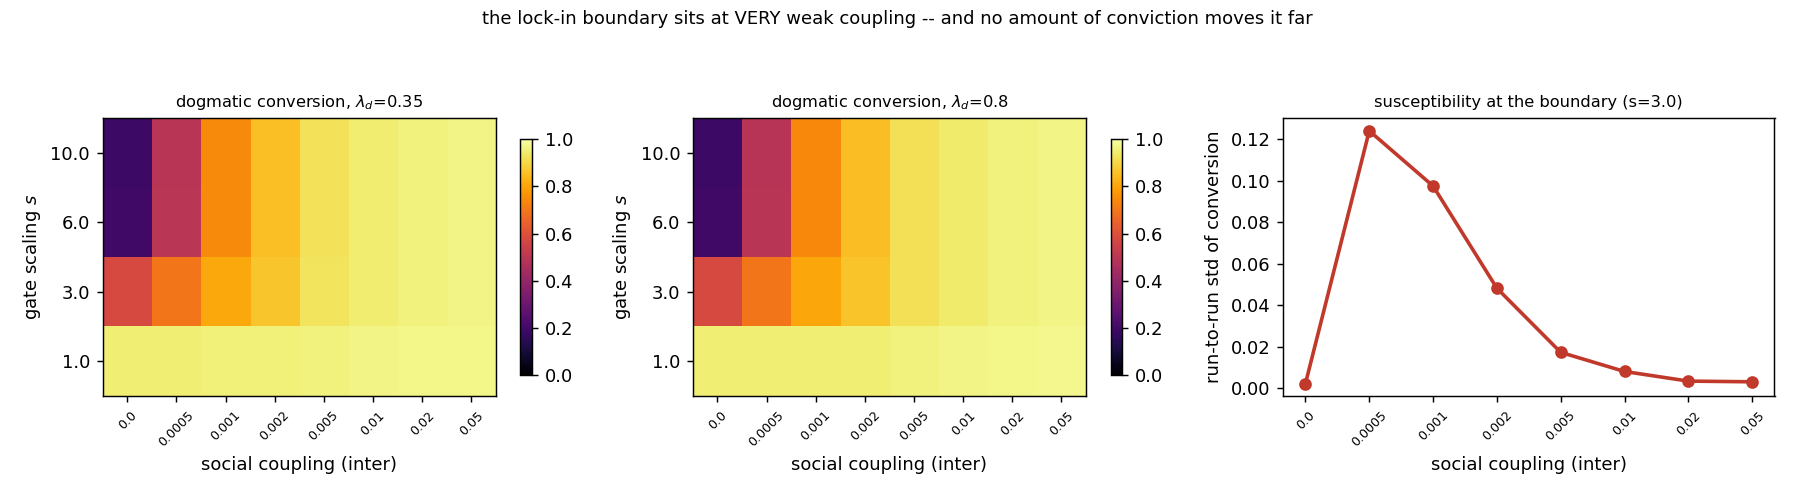
\includegraphics[width=0.85\linewidth]{fig_kuhn_lockin_boundary.png}
\caption{Only isolation protects a superseded paradigm (phlogiston sweep, fixed trust).
\emph{Left, centre:} the fraction of the dogmatic community that converts to oxygen, as a
function of contact (\emph{inter}) and of how strongly conviction gates disconfirming channels
($s$), at two conviction levels ($\lambda_d=0.35$ and $0.8$). Past
\emph{inter}$\,\approx0.005$ nearly everyone converts, and doubling conviction barely changes
the picture. \emph{Right:} the run-to-run spread spikes in a narrow band around
\emph{inter}$\,\approx5\times10^{-4}$: a sharp boundary, not a fade.}
\label{fig:res-lockin}
\end{figure}

\paragraph{Pooling kills the lone discoverer---by protocol, not by principle \emph{(earlier
prototype)}.}
In the prototype, discovery means waking a node---oxygen---that no agent's network yet
contains; candidates arrive at a Poisson rate $r$ and are accepted on the model log Bayes
factor (Appendix~\ref{app:crisis-discovery}), so the fraction that discovers follows the
waiting-time law. What the protocol governs is \emph{survival}: delta pooling reads
\emph{has no such variable}---a fact about an agent's model class---as \emph{maximally
certain it is zero} \citep{genest1986,friston2023federated}, so a discovery made by one
agent at a time is averaged away every round, and staggered survival is zero at every rate.
Under dimension-aware \emph{abstention} pooling---each precision entry pooled only over the
neighbours that represent it---the survival threshold relocates wholesale: survival tracks
the discovery fraction itself ($0.39/0.64/0.86$ at $r_0=0.005/0.01/0.02$;
Fig.~\ref{fig:res-fusion}).

\begin{figure}[h!]
\centering
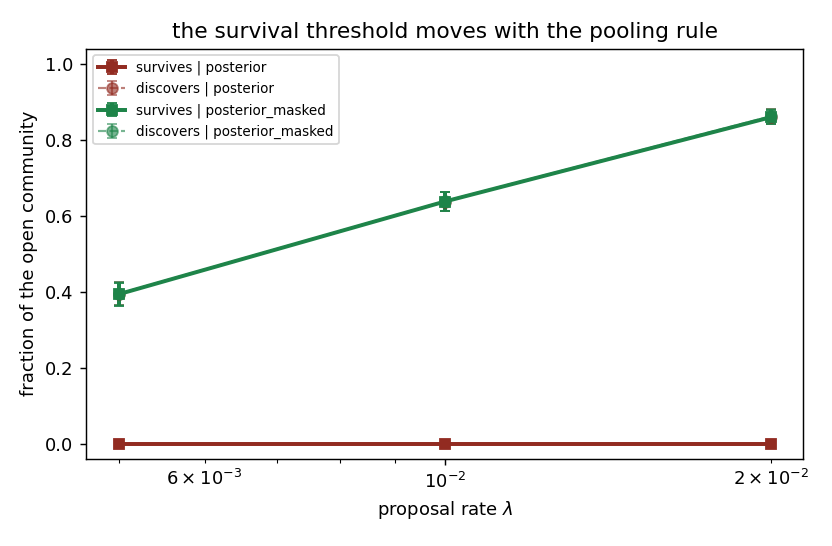
\includegraphics[width=0.62\linewidth]{fig_kuhn_fusion.png}
\caption{The survival threshold moves with the pooling protocol (32 seeds per cell). Solid:
fraction of the open community whose concept survives; dashed: fraction that discovers at all.
Under delta pooling (red) a pinned slot is a confident ``no such thing'' and staggered survival
is zero at every rate; under abstention pooling (green) survival tracks discovery.
Incommensurability as a population-level force is a property of the protocol, not of the
concepts.}
\label{fig:res-fusion}
\end{figure}

\paragraph{Every escape goes around the averaging, never through it \emph{(earlier
prototype)}.}
Four mechanisms were layered on the prototype baseline, and none lets two connected
communities holding the same data \emph{remain} in disagreement. An adequacy-inferred
proposal rate---look harder when the residual is high---shortens crisis-to-discovery from
$55$ to $29$ steps, matched by a constant rate of equal mean: it re-times the passage.
Social excitation (a Hawkes kernel on neighbours' discoveries) collapses the waking
dispersion from $64$ to $2$ steps and lifts staggered survival from $0$ to
$0.88$--$0.95$: synchrony outruns the averaging rather than escaping it. An audited
wake-then-prune cycle re-pins $100\%$ of wakes in the null world: curiosity kept honest,
nothing else changed. Value accretion---conviction grown from inside by each
confirmation---delays conversion ${\sim}2.2\times$ and never prevents it: time bought, not
immunity. Each either re-times the passage through the consensus bottleneck or synchronizes
the population for it.

\paragraph{Robustness and controls \emph{(earlier prototype)}.}
The arc is robust across forgetting and observation noise ($\omega\in[0.9,1.0]$,
$\sigma_o\in[0.25,1.0]$): crisis and reduction survive everywhere---including the
no-forgetting wall $\omega=1$, where only discovery thins: a community that never forgets
still sees its paradigm die, but loses the capacity to grow the successor. Each experiment
ships its own null and positive controls---a world that never shifts produces neither crisis
nor discovery; the gated, isolated community stays locked; Poisson discovery follows the
waiting-time law---and no acceptance bar is tuned anywhere: the wake's sole accept test is
the model log Bayes factor (Appendix~\ref{app:crisis-discovery}); whatever the derivations
there do not fix is named there as a commitment.

% ======================================================================
\section{Inferred reliability and represented rivals: definitions and experiment details}
\label{app:reliability}
% ======================================================================

This appendix carries the exact definitions of the two mechanisms Result 2
(\S\ref{sec:res-distinct}) turns on---the Student-$t$ reliability gate in its three reads
(channels, opinions, wiring) and the represented-rival architecture ($K$ candidate nets,
prequential scoring, hypothesis-aligned fusion)---and then walks through every gated
experiment behind the quoted numbers: what was set up, what to look at, and what each
headline figure means. Consult it whenever a main-text claim cites a gate or a wall; the
closing paragraph states the three commitments that bound all of it.

\paragraph{The three reads of one functional.}
Every gate in the paper is the Student-$t$ scale-mixture weight
$\eta=(\nu+1)/(\nu+z^2)$---the posterior expectation of a source's latent noise scale given
its standardized squared surprise $z^2$ (one E-step of the EM view of $t$-regression)---applied
to three different surprises. \emph{Channels:} $z_k^2=(o_k-(H\mu)_k)^2/\mathrm{predvar}_k$ with
$\mathrm{predvar}_k=\sigma_o^2+(H\Pi^{-1}H^{\!\top})_{kk}$, the agent's own surprise at
observation $k$ before depositing it; $\eta_k$ multiplies the channel's deposit, composing
with the conviction gate of \S\ref{sec:revision}. \emph{Opinions:}
$z_{ij}^2=\sum_v(\mu_j[v]-\mu_i[v])^2/(\Pi_i[v,v]^{-1}+\Pi_j[v,v]^{-1})$, the calibrated
disagreement of two posteriors summed over the measured nodes (summed, not averaged: a localized
heresy must be able to sever trust); $\eta_{ij}$ multiplies the fusion weights, whose row
normalization absorbs the overall scale. \emph{Wiring:} the same sum taken over contested
coupling entries $x=\Pi[a,c]$, normalized by their pairwise symmetric scale
$\max((x_i^2+x_j^2)/2,\,\epsilon^2)$---bounded per coupling, and invariant to the global
precision growth the forgetting equilibrium produces, so it reads \emph{how} two agents wire
the world, not how much evidence they hold.

\paragraph{Represented rivals: definitions.}
Each agent carries $K$ candidate nets $(\Pi_{ik},h_{ik})$ and log-weights $L_{ik}$ over a
model index. Per step, every candidate is scored by its prequential predictive density
\emph{before} the shared deposit lands, $\log p(o_t\mid o_{<t},M_k)$, so
structure-discriminating evidence accumulates in $L$ rather than being erased by the Fisher
deposit (which never sees the observation's value). Fusion is hypothesis-aligned---candidate
$k$ pools only with neighbours' candidate $k$---and the log-weights pool log-linearly with
damping $\alpha_m$: $L\leftarrow(1-\alpha_m)L+\alpha_m WL$. Deviations of the pooled log-odds
from the population mean converge to $(I-W)^{+}(s-\bar s)/\alpha_m$, a constant gap of
${\sim}\,s/2\alpha_m$ nats for two symmetric camps: a genuine fixed point---the wall of
Fig.~\ref{fig:res-walls}---whose height the early-measured per-step source predicts
conservatively (realized $110$ nats at the horizon, tail still growing at $+0.016$ nats/step).
Anchored forgetting on the candidate nets,
$\Pi_{ik}\leftarrow\Pi_{0k}+\omega(\Pi_{ik}-\Pi_{0k})$, is part of the mechanism: without it
every candidate's precision grows without bound and their predictive densities converge. $K=1$
reduces exactly to plain fuse-then-observe, which is how the Gaussian baselines run on
byte-identical observation streams; each architecture runs its own best memory setting.

\begin{figure}[h!]
\centering
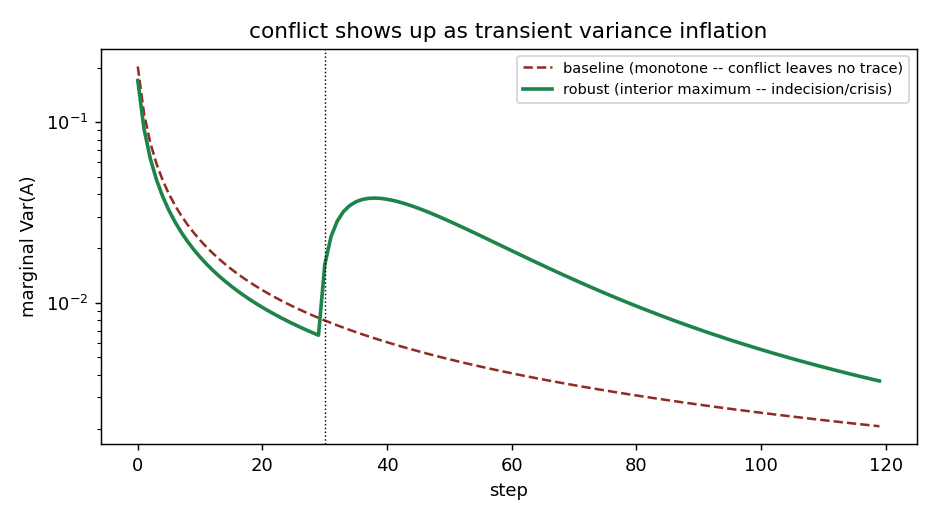
\includegraphics[width=0.52\linewidth]{fig_abc_variance.png}
\caption{Conflict as suspended confidence (\S\ref{sec:res-distinct}). A channel turns
contradictory at step 30. The Gaussian baseline (dashed) grows monotonically more
certain---the Gaussian confident compromise; the gated agent's variance (solid) shows an
interior maximum: doubt rises while data accumulate, then resolves.}
\label{fig:res-variance}
\end{figure}

\paragraph{The experiments, interpreted.}
All runs are seeded, assertion-checked at run time, and write their summary statistics next
to their figures. The main-text experiments first. \emph{Conflict crisis}
(\S\ref{sec:res-distinct}): one agent on a three-commitment chain whose channel $A$ turns
contradictory at $t{=}30$ ($\nu{=}4$, $T{=}120$). Watch the posterior variance
(Fig.~\ref{fig:res-variance}): the gate infers the channel unreliable ($\eta_A\to0.16$) and
the variance peaks at $t{=}38$---doubt rising while data accumulate, the interior maximum no
Gaussian can produce---while the violated edge carries $5.3\times$ the strain of its
neighbours, so the agent also knows \emph{where} it is torn. \emph{Divergent wiring}
(\S\ref{sec:res-distinct}): $N{=}60$ in a structurally underdetermined world, two attention
camps, five seeds. The number to read is surviving cross-community structure: fixed
trust retains $10\%$ of the disconnected benchmark, the
opinion-reading gate $10.2\%$ (the camps agree in means, so it never fires), the
wiring-reading gate $94\%$---what matters is \emph{which} disagreement a gate can see, not
that there is one. \emph{Rival lock-on} (\S\ref{sec:rivals}): one agent, $K{=}2$ wirings
differing in nothing but structure ($T{=}400$): the prequential log-weights separate at
$0.13$ nats/step and $q(M_1)\to1.0$, while the Gaussian pool's half-strength blur stays
frozen ($<10^{-3}$ drift)---the rival layer decides a question the pooled net cannot ask.
\emph{The wall} (\S\ref{sec:res-distinct}): $N{=}16$, two camps, full contact, theory-laden
channels ($T{=}1500$, five seeds): end-of-run disagreement $2.5\times10^{-4}$ plain, $0.075$
gated, $2.79$ rival, with $q_{\mathrm{own}}=1.0$ in both camps---the fixed-point gap of
Fig.~\ref{fig:res-walls}, held, not decaying. \emph{Targeted reduction}: one agent, a chain
with one world-violated coupling ($T{=}80$): the violated edge is top-strain at every step
and the $\Delta F$ verdicts are correct from step 1---reduction points where the world
disagrees.

\paragraph{Population-level readings of the same gates.}
Four further runs put the gates through the full Kuhnian cycle; each is a further reading of
the same two results---homogenization delayed, never escaped---and is reported here rather
than in the main text. \emph{Crisis trace} ($N{=}20$, world flips at $t{=}40$, $\nu{=}2$,
$T{=}800$): the community first \emph{denies}---mean channel weight $\bar\eta$ falls from
$0.85$ to $0.17$ and conversion stalls $4.3\times$---then \emph{rehabilitates} the doubted
channel ($\bar\eta\to1.27$) once the revised wiring fits it, agreement channels staying
$>0.85$ throughout: denial and rehabilitation as one gate's trajectory. \emph{Gated camps}
($N{=}20$, complete graph, opposed camps, $\nu_s{=}0.5$, $T{=}80$): uniform fusion preserves
$0.1\%$ of initial disagreement, the gated run $48\%$, cross-camp trust collapsing to
$0.8\%$ of within-camp---self-organized isolation. \emph{Schism threshold} (same setup,
sweeping prior confidence at contact): fixed trust ends $\le0.2\%$ everywhere; the gate is
inert below a confidence threshold ($<1\%$) and holds $17/48/76\%$ above it---schism feeds
on accumulated conviction. \emph{Lock-in rerun} ($N{=}80$, full cycle, $\nu_s{=}0.5$,
$T{=}180$, \emph{inter} swept): conversion half-time stretches $78\to146$--$170$ and
conversion drops to $0.54$--$0.73$ versus $0.92$ under fixed trust, because cross-community
trust first collapses ($<1\%$) and is later restored ($>90\%$): isolation self-organized,
then self-undone---delay without escape.

\paragraph{The transition's shape is the wiring's signature.}
A final run replays the Kuhnian transition of \S\ref{sec:res-kuhn} where it must
\emph{spread}: $N{=}24$, a vanguard of $4$ keeps full attention on the disconfirming
experiment while the rest self-censor it ($\gamma{=}0.99$, a trickle), on the four
reference contact graphs of network epistemology---cycle, wheel, two communities,
complete (the topology dial of Table~\ref{tab:dials}; $50$ seeds each). Every
community completes the transition---at a trickle there is no speed/accuracy trade to
pay \citep{zollman2010}---but the \emph{same} world flip arrives as four different
events (Fig.~\ref{fig:res-trajtopo}): a synchronized flip on the complete graph (the
median conservative converts at $t{=}220$, inter-agent spread $4$ steps), a hub
broadcast on the wheel ($t{=}232$, spread $11$: the vanguard holds the hub, so
conversion arrives everywhere at once despite a $\lambda_2$ an order of magnitude
below the complete graph's---centrality, not density), a staircase across the
community bridge ($t{=}453$, spread $57$), and a travelling wave around the cycle
($t{=}488$, spread $102$: revolution reaches each agent as a \emph{date}, not an
event). Same gates, same evidence, same candidates---the shape of a paradigm shift is
a property of the contact graph.

\begin{figure}[h!]
\centering
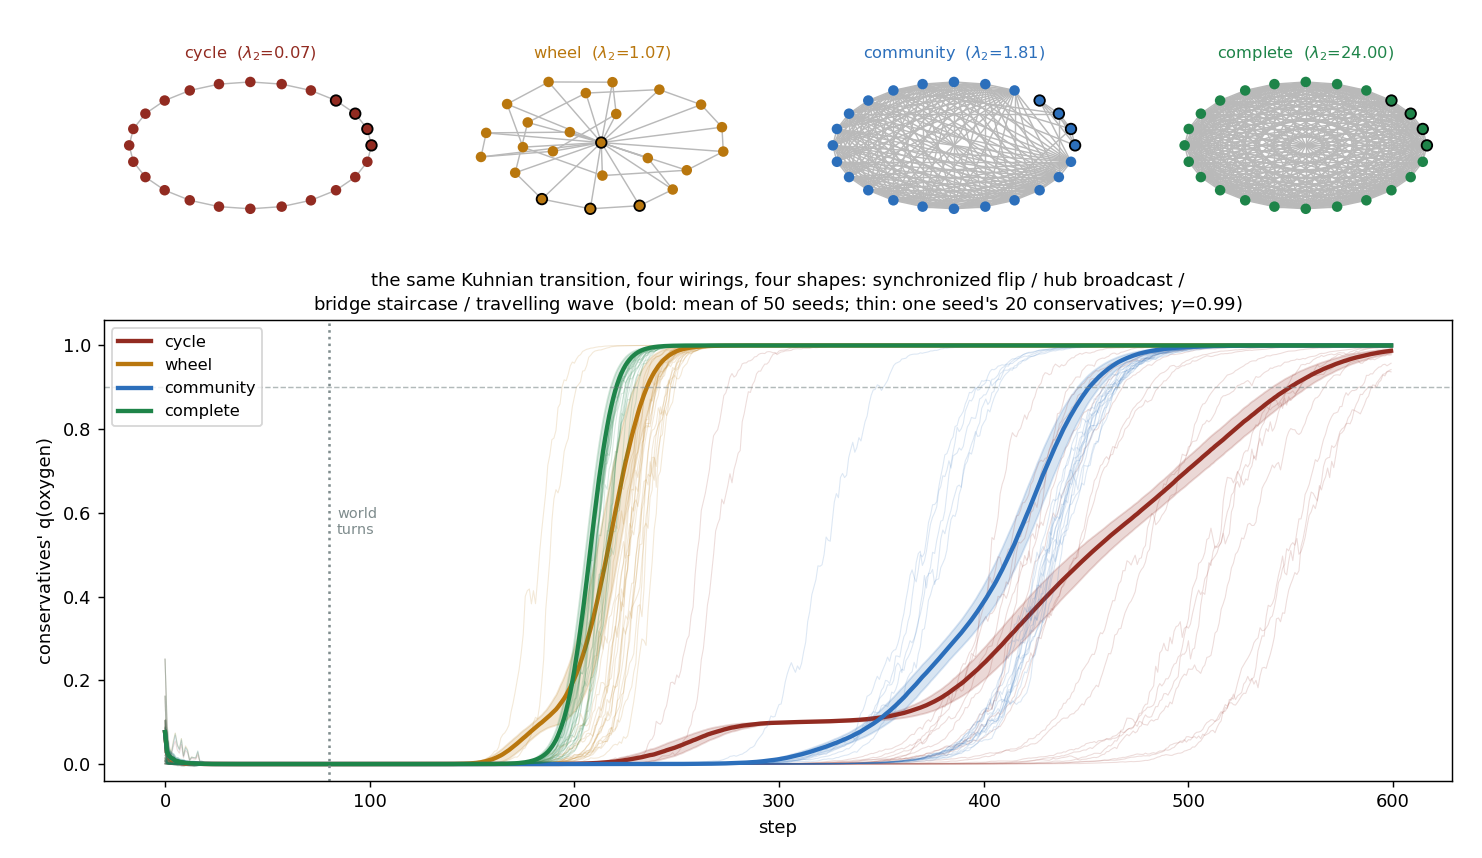
\includegraphics[width=0.92\linewidth]{fig_kuhn_trajectories_by_topology.png}
\caption{The same Kuhnian transition on four contact graphs, on one canvas. Bold:
conservatives' mean $q(\mathrm{oxygen})$ ($50$ seeds $\pm$ s.d.); thin: one seed's
$20$ conservative agents; the world turns at the dotted line; vanguard nodes are
outlined in the glyphs. Complete and wheel flip together and early; the two-community
graph converts as a staircase after the bridge delay; the cycle converts as a
travelling wave---the per-agent fan is the wiring's signature.}
\label{fig:res-trajtopo}
\end{figure}

\paragraph{Scope, stated plainly.}
Three commitments bound the results. (i) Both gates are \emph{memoryless}: $\eta_k$ and
$\eta_{ij}$ are instantaneous functions of current surprise, so every school and schism reported is
metastability relative to a horizon, not a new fixed point---the contraction theorem owns
$t\to\infty$, and the lock-in rerun shows the trade directly: a harsher gate ($\nu_s{=}0.2$)
holds the boundary longer but leaves its own undoing unfinished at the same horizon, because
the lock and the merge run on the same clock. (ii) The schism control is normalized by the
pre-contact stance gap, since one uniform fusion step collapses the fixed-trust camps before
the first logged sample. (iii) Structure-as-precision-pattern is attention-driven in the
linear-Gaussian class (the Fisher deposit $H^{\!\top}\mathrm{diag}(w)H/\sigma^2$ never sees the
observation's value): a camp committed to a wiring the data do not support consolidates it
exactly as strongly as the supported camps do, so the wiring gate can protect a pluralism but
cannot tell a supported school from a merely committed one---the data's verdict on an
unsupported theory lives in the means, and in the strain and reliability reads that live on
them. This refuted our own prediction, and it is the right caveat on every wiring-gate claim.

% ======================================================================
% The crisis and discovery checks, derived from the ledger (+ the
% exploration-as-social-process mechanism readings at its tail).
% ======================================================================
% APPENDIX (v5): the crisis check derived from the ledger, the Schur
% residue (moved here from the operator appendix), and the prototype's
% discovery check in compressed form.
% \input from changing_networked_mind_v5.tex (after the reliability appendix).
% Uses the main paper's macros (\Top, \KL, \Eq) and labels (eq:tilted,
% eq:bmr, eq:gamma, sec:structurelearning, sec:revision, tab:dials).
% ======================================================================

% ----------------------------------------------------------------------
\section{The crisis check, the Schur residue, and the prototype's discovery check}
\label{app:crisis-discovery}
% ----------------------------------------------------------------------

This appendix derives the simulation's threshold events from the single objective the paper
already carries, so that no structural change reads as a stipulated event. The \emph{crisis
check}---step 3 of the loop in \S\ref{sec:model}, the only structural move the model of this
paper makes---is derived in full. The \emph{Schur residue} comes next: what marginalizing a
hub leaves behind, the algebra behind both the oxygen rival of Appendix~\ref{app:null} and
the discovery direction. The \emph{discovery check} belongs only to the earlier prototype of
Appendix~\ref{app:null} (the main-text model runs reduction only,
\S\ref{sec:structurelearning}) and is derived in compressed form so the prototype's flagged
numbers remain auditable; whatever is \emph{not} derived is named as a commitment at the
end.

\subsection{One ledger for every structural move}

The bounded agent of \S\ref{sec:revision} revises its beliefs by minimizing
$\KL{q}{p(x\mid o,G)}-\lambda\,\Eq{q}{U^{\!\top}\!x}$ (Eq.~\ref{eq:tilted}): fidelity to the
honest posterior, traded against the value of where the commitments land, at temperature
$\lambda$. A structural move---pruning an edge, waking a node---changes both terms, so the same
objective scores the move:
\begin{equation}
\mathrm{score}(M\!\to\!\tilde M)
\;=\;
\underbrace{\Delta F}_{\text{log Bayes factor}}
\;+\;
\underbrace{\Delta G}_{\text{epistemic gain}}
\;+\;
\lambda\,\underbrace{\Delta U}_{\text{conviction value}},
\qquad
\text{accept}\iff \mathrm{score}>0,
\label{eq:ledger}
\end{equation}
with $\Delta F$ the evidence for the edited structure, $\Delta G$ the expected information gain
about any newly introduced latent (zero for a prune), and
$\Delta U = \Eq{q_{\tilde M}}{U^{\!\top}\!x}-\Eq{q_{M}}{U^{\!\top}\!x}$ the change in the
conviction-field value of the commitments. Equation~\eqref{eq:ledger} is not a new mechanism:
it is Eq.~\eqref{eq:tilted} evaluated at two structures and differenced. Both threshold events
below are instances of it.

\subsection{The crisis check is the ledger on a prune}

For a prune, every term of Eq.~\eqref{eq:ledger} is closed-form in the linear-Gaussian setting.
The evidence half is Bayesian model reduction (Eq.~\ref{eq:bmr}): writing the agent's
accumulated likelihood deposit as $J=\Pi-\Pi_0$, $j=h-h_0$, the Savage--Dickey identity scores
the swap of the prior $(\Pi_0,h_0)$ for the edge-$e$-reduced prior $(\Pi_0^{(e)},h_0^{(e)})$
under the same likelihood, and---this is the part the main text does not spell out---it
\emph{already exhibits the reduced posterior},
\begin{equation}
\Pi^{(e)} = \Pi_0^{(e)} + J,
\qquad
h^{(e)} = h_0^{(e)} + j ,
\end{equation}
so the value half costs one linear solve per candidate edge:
\begin{equation}
\Delta U_e \;=\; U^{\!\top}\!\bigl(\mu^{(e)}-\mu\bigr),
\qquad
\mu^{(e)} = \bigl(\Pi^{(e)}\bigr)^{-1}h^{(e)},\quad \mu = \Pi^{-1}h,
\label{eq:dU-prune}
\end{equation}
with $U=\Top u$ the agent's \emph{current} conviction field, read along its present couplings.
The crisis check is then exactly the ledger: edge $e$ is flagged iff
$\Delta F_e + \lambda\,\Delta U_e > 0$, and \emph{crisis} is the round at which both protective
belt edges are flagged, upon which the agent adopts the reduced prior composed over every edge
its own ledger flags (the hub released). Pruning a conviction-protective edge moves the
posterior mean away from the cherished commitments, so $\Delta U_e<0$ and the rule reproduces
the intuitive form ``the evidence must overcome $\lambda$ times the value the edge protects.''

A natural surrogate suggests itself here: the static threshold $\Delta F_e > \lambda\,v_e$ with
$v_e = |U_{\mathrm{parent}}|+|U_{\mathrm{child}}|$, the summed conviction magnitude at the
edge's endpoints---available without a solve, and with the
right \emph{form} (it is Eq.~\eqref{eq:ledger} with $\Delta U_e \equiv -v_e$). But it has the
wrong \emph{content}: $v_e$ is a static stand-in for a quantity the model can compute exactly,
so we compute it. The difference is not cosmetic, and its direction is itself informative:
because the reduced and full posteriors share the likelihood deposit, the mean displacement of
a prune---and with it $\lambda\,\Delta U_e$---\emph{shrinks as evidence accumulates}. A
data-rich paradigm is barely protected at the threshold; almost all of its persistence must
come from upstream, from the conviction gate that decides which evidence is allowed to
accumulate at all (Eq.~\ref{eq:gamma}). The static surrogate would quietly overstate threshold
protection; the exact ledger locates lock-in where the paper's results put it: gating plus
isolation, not a high bar at the moment of decision.

\subsection{The Schur residue: what marginalizing a hub leaves behind}

Marginalizing a hub condenses its influence into new edges among its neighbours: for a
common-cause structure over $(x_1,x_2,b)$,
\begin{equation}
\Pi=\begin{pmatrix}2&0&1\\0&2&1\\1&1&2\end{pmatrix}
\ \xrightarrow{\ \text{marginalize } b\ }\
\begin{pmatrix}2&0\\0&2\end{pmatrix}-\tfrac12\begin{pmatrix}1\\1\end{pmatrix}\begin{pmatrix}1&1\end{pmatrix}
=\begin{pmatrix}1.5&-0.5\\-0.5&1.5\end{pmatrix},
\label{eq:schur}
\end{equation}
a direct coupling induced where the joint had a zero. Conditioning on a shared \emph{effect} is the
dual operation: two commitments that jointly feed one observation are a priori independent, and
clamping that observation anti-couples them---explaining away, run on the precision matrix. Both
operations fill in the off-diagonal coupling the carry-over cost $\kappa=\Top\bone$ is built
from, and Fig.~\ref{fig:schur-generic} draws both on the smallest nets that exhibit them.

Two of the paper's objects are instances of this residue. The oxygen rival of
Appendix~\ref{app:null} keeps exactly the direct mass-law couplings that marginalizing the
phlogiston hub leaves behind---the incumbent's Schur complement over its hub, means
corrected. Read in reverse, the residue is a \emph{signature}: a hidden hub $b$ with
couplings $c$ leaves, on marginalization, the rank-one footprint $-cc^{\!\top}/\Pi_{bb}$ in
the visible precision---exactly what the prototype's discovery check reads off the residual
below.

\begin{figure}[h!]
\centering
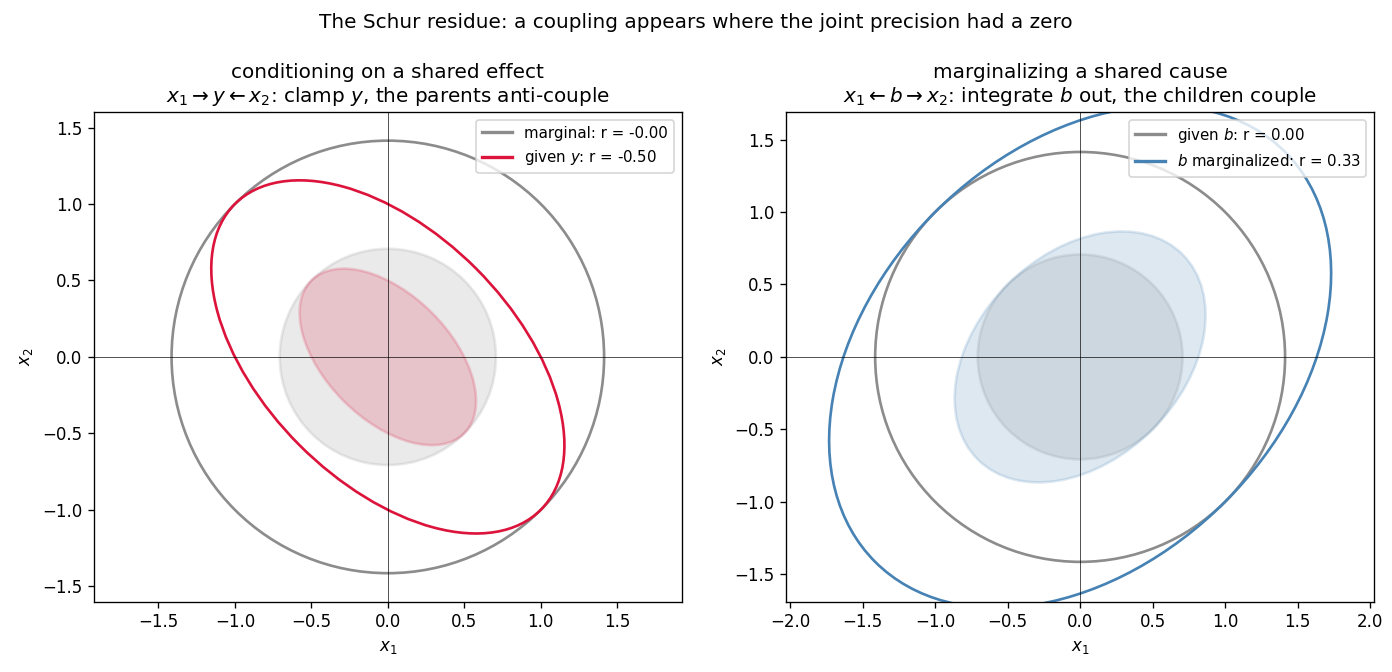
\includegraphics[width=0.60\linewidth]{fig_schur_generic.png}
\caption{The Schur residue, computed on the smallest nets that show it. \emph{Left:} conditioning
on a shared effect ($x_1\!\to\!y\!\leftarrow\!x_2$): the parents are a priori independent (grey,
$r=0$); clamping their common descendant $y$ manufactures an anti-correlation (crimson,
$r=-0.50$)---explaining away. \emph{Right:} marginalizing a shared cause (the matrix of
Eq.~\ref{eq:schur}): the children are independent given $b$ (grey); integrating $b$ out leaves
them coupled (blue, $r=+0.33$). In both cases a coupling appears where the joint precision had a
zero---the off-diagonal mass the carry-over cost $\kappa=\Top\bone$ is built from.}
\label{fig:schur-generic}
\end{figure}

\subsection{The discovery check is the ledger on an expansion (prototype only)}

This check runs only in the earlier phlogiston prototype of Appendix~\ref{app:null}; the
model of the main text runs reduction only (\S\ref{sec:structurelearning}). Expansion cannot
be closed-form: a new node needs a real inversion, and---Stanford's problem of unconceived
alternatives---the agent cannot plan toward a dimension it has not conceived. The check
therefore has exactly two parts, and only two:

\begin{enumerate}
\item \textbf{Arrival.} Candidate proposals arrive at a Poisson rate $r$. This is the one
place a stipulated process enters, and it is a deliberate modelling commitment: a rate is the
maximally agnostic model of conceiving what one has not conceived. The proposal's
\emph{direction} is read from the model's own prediction errors: by the rank-one footprint
above, the leading eigenvector of the windowed error second moment is the best single-hub
explanation of the residual. The window is an estimator horizon, not a gate.
\item \textbf{Acceptance.} The arrived proposal is accepted iff the model log Bayes factor of
the bordered (hub-wired) model against the agent's current one is positive---iff the residual
genuinely loads on the proposed hub. The epistemic gain $\Delta G$ sits on the other side of
the move: being positive for \emph{any} new latent, it pays for \emph{attempting} the
inversion, and it cannot keep a hub the data do not hold---an accept test that included it
would wake on pure noise. Entertaining is paid by curiosity; keeping is paid by evidence.
Repeated looks give the Bayes factor a small false-discovery rate, owned rather than hidden;
its principled remedy is the audited wake-then-prune cycle of Appendix~\ref{app:null}, not a
reinstated threshold.
\end{enumerate}

A tempting third part is deliberately absent: a \emph{trigger}, requiring the residual floor
(the eigenvalue above) to clear some height before the Bayes factor is consulted. It would
duplicate the accept test's job with a free constant, so the check has no tuned threshold:
the rate carries Stanford's commitment, the eigenvector the direction, the ledger decides.
(The floor is recorded as telemetry: the visible signature of the residual the old paradigm
had been absorbing.)

\subsection{What remains a modelling commitment}

The derivations leave a short list of choices not forced by the formalism; the claim that
``crisis, revolution and discovery are threshold crossings of the model's own evidence'' is
honest only with this boundary drawn:

\begin{itemize}
\item \textbf{The belt conjunction.} ``Crisis'' is operationalized as \emph{both} named
mass-law edges flagged in the same round. The per-edge accept is derived; the conjunction over
those two edges is our operational definition of having eliminated the phlogiston mass-law
reading.
\item \textbf{The ordering --- a result, not a commitment.} The prototype attempts expansion
only after an agent's own crisis, but the ordering is enforced by the evidence rather than by
fiat: running the identical proposal + ledger pipeline for every pre-crisis agent at every
step (without applying it), the ledger rejects $13{,}180$ of $13{,}185$ pre-crisis
agent-steps, and the five crossings are marginal ($\Delta F < 0.005$)---the repeated-look
false-positive rate owned above. The intact paradigm absorbs the residual; there is nothing
for the check to find until reduction exposes it.
\item \textbf{The Poisson rate $r$} (swept), the prediction-error \emph{window} (an estimator
horizon), a short \emph{warm-up} before reduction is permitted (an initialization guard), and
the released hub's self-precision are quantitative choices of the same standing as the other
prototype dials of Table~\ref{tab:dials}.
\end{itemize}

% ----------------------------------------------------------------------


\end{document}
